%=======================================================================
%  paper.tex
%  "Matching Algorithm Families to Problem Structure:
%   An Empirical Comparison of Search, Constraint Satisfaction,
%   and Learning-Based Optimization"
%
%  Self-contained arXiv (cs.AI) preprint source.
%  Compile:  pdflatex paper.tex   (run twice for cross-references)
%  No bibtex needed: the bibliography is embedded as thebibliography.
%  A companion references.bib is provided if you prefer natbib/bibtex.
%=======================================================================
\documentclass[10pt]{article}

% arXiv's format guideline asks for a 1in minimum margin; 0.85in (used
% earlier) is under it. The extra whitespace costs roughly one page, which
% arXiv does not care about -- there is no page limit.
\usepackage[a4paper,margin=1in]{geometry}
\usepackage[T1]{fontenc}
\usepackage{lmodern}
\usepackage{amsmath,amssymb}
\usepackage{graphicx}
\usepackage{booktabs}
\usepackage{xcolor}
\usepackage{caption}
\usepackage{subcaption}
\usepackage{enumitem}
\usepackage{microtype}
\usepackage[hidelinks]{hyperref}
\usepackage{url}

\graphicspath{{figures/}{./figures/}{.}}
\captionsetup{font=small,labelfont=bf}
\setlength{\parskip}{2pt}

% --- Float management -------------------------------------------------
% This paper carries 11 figures and 6 tables in a single-column layout. With
% LaTeX's stock float parameters (topnumber=2, totalnumber=3, and only 18
% float slots) the floats queue up, get deferred past their sections, and
% the run can die with "Too many unprocessed floats" -- which is why
% figures appeared to be missing. Relax the limits and enlarge the store.
\usepackage{placeins}
\makeatletter\@ifundefined{extrafloats}{}{\extrafloats{100}}\makeatother
\setcounter{topnumber}{3}
\setcounter{bottomnumber}{2}
\setcounter{totalnumber}{5}
\renewcommand{\topfraction}{0.92}
\renewcommand{\bottomfraction}{0.7}
\renewcommand{\textfraction}{0.06}
\renewcommand{\floatpagefraction}{0.65}
% Tables: tighter inter-column padding keeps wide tables inside the text block.
\setlength{\tabcolsep}{4pt}
% Shrink an over-wide table to the text width, but NEVER enlarge a narrow one
% (plain \resizebox scales both ways and blows small tables up). In one-column
% layout \columnwidth == \textwidth, so this now fits to the full text block.
\newcommand{\fitcol}[1]{%
  \resizebox{\ifdim\width>\columnwidth\columnwidth\else\width\fi}{!}{#1}}

% --- Keep run-in headings attached to their text ----------------------
% A \paragraph{...} that lands at the foot of a column is left stranded
% with its body on the next page. Require enough room for the heading
% plus the first few lines, otherwise move the whole unit forward.
\usepackage{needspace}
\let\akparagraph\paragraph
\renewcommand{\paragraph}[1]{\Needspace*{4\baselineskip}\akparagraph{#1}}
\clubpenalty=10000      % no orphan lines
\widowpenalty=10000     % no widow lines
\displaywidowpenalty=10000

\title{\vspace{-1.2em}\textbf{Matching Algorithm Families to Problem Structure:\\
An Empirical Comparison of Search, Constraint Satisfaction,\\
and Learning-Based Optimization}}

\author{%
  \normalsize Shraban Karmoker Avi\thanks{Corresponding author: \texttt{shrabankarmoker-2021911220@cs.du.ac.bd}}
  \quad and\quad \normalsize [Supervisor Name]\\[2pt]
  \small Department of Computer Science and Engineering\\
  \small University of Dhaka, Dhaka, Bangladesh
}
\date{}

\begin{document}
\maketitle

\begin{abstract}
\noindent
Modern artificial intelligence offers a wide toolbox---uninformed and informed
state-space search, constraint satisfaction, population-based metaheuristics,
dynamic programming and reinforcement learning---yet practitioners often reach
for a familiar algorithm rather than the one the problem actually calls for.
This paper argues, and empirically demonstrates, a single organizing principle:
\emph{the structural properties of a problem determine which family of algorithms
is appropriate}. We test this thesis on three deliberately dissimilar decision
problems, each implemented from scratch and evaluated under a common,
reproducible protocol. \textbf{(i)} An urban route-finding task exposes the gap
between uninformed and informed search: A$^\star$ attains the optimal path cost
while expanding up to $17\%$ fewer nodes than uniform-cost search, whereas greedy
best-first search is the cheapest to run ($11$ expansions) but loses optimality
once edge weights shift. \textbf{(ii)} A fuel-rationing task, cast as a
constraint satisfaction problem with $11$ constraints and a $720^{n}$ raw search
space, shows a sharp phase transition: at a fully saturated instance ($n{=}40$)
naive backtracking exhausts its node budget after $2461$ backtracks, while adding
the minimum-remaining-values heuristic solves the same instance in $41$ nodes
with zero backtracking. \textbf{(iii)} A smart-agriculture pipeline combines
combinatorial optimization (assigning $400$ flowers to $5$ robots, a $5^{400}$
space) with sequential decision-making under uncertainty (grid navigation with
stochastic actuation). A genetic algorithm outperforms particle swarm
optimization on the discrete allocation ($1.43$ vs.\ $1.60$ fitness, over $10$
seeds), and a model-free Q-learning agent rediscovers a statistically
indistinguishable navigation policy ($59.1$ vs.\ $59.1$ mean reward) that value
iteration computes $176\times$ faster when a model is available. Across all three case studies the same lesson
holds: exact methods dominate when the space is small and known, inference and
heuristics rescue tractability at the constraint-satisfaction phase transition,
and population-based or learning methods become the only viable option once the
space is enormous or the environment is unknown. We release all code, fixed-seed
experiment scripts and figures to make every number reproducible.
\end{abstract}

\smallskip
\noindent\textbf{Keywords:} heuristic search, A$^\star$, constraint satisfaction,
backtracking, particle swarm optimization, genetic algorithms, value iteration,
Q-learning, reproducibility.

%=======================================================================
\section{Introduction}
%=======================================================================
A recurring failure mode in applied artificial intelligence is \emph{method
fixation}: selecting an algorithm because it is familiar or fashionable rather
than because it fits the problem. Yet the classical AI literature has long
organized its methods around problem structure---state-space search for
path-finding, constraint propagation for combinatorial feasibility,
metaheuristics for rugged high-dimensional optimization, and Markov decision
processes for sequential control under uncertainty~\cite{russell2020,
pearl1984,dechter2003,sutton2018}. What is often missing, especially in
educational and early-research settings, is a single, controlled demonstration
that ties these families back to the structural cues that should trigger them.

This paper provides exactly that demonstration. Our central claim is deliberately
simple:

\begin{quote}\itshape
The structure of a problem---the size and observability of its state space, the
presence of hard constraints, the shape of its objective, and whether outcomes
are deterministic---dictates which family of algorithms is appropriate.
\end{quote}

\noindent
We support the claim not by argument alone but by three implemented,
instrumented case studies chosen to span sharply different structures
(Table~\ref{tab:overview}). Each is a self-contained problem with a real-world
framing (two set in the road network of Dhaka, Bangladesh; one in an autonomous
greenhouse), each is implemented from first principles in Python/NumPy with no
black-box solver, and each is run under a fixed random seed so that every
reported quantity---timings aside---reproduces exactly.

\begin{table}[t]
\centering
\caption{The three case studies span deliberately different problem structures.
Each stresses a different family of algorithms.}
\label{tab:overview}
\small
\renewcommand{\arraystretch}{1.25}
% Widths sum to 14.4cm; \tabcolsep adds 1.27cm, for 15.67cm against the
% 15.93cm \textwidth that a4paper+1in margins leaves. Sized for that margin.
\begin{tabular}{@{}p{2.7cm} p{3.3cm} p{4.3cm} p{4.1cm}@{}}
\toprule
& \textbf{CS-1: Route finding} & \textbf{CS-2: Fuel rationing} & \textbf{CS-3: Smart agriculture} \\
\midrule
Core question & \emph{Which} path to the goal? & \emph{Which} assignment satisfies all rules? & \emph{Which} robot gets which task, and \emph{how} does it move? \\
Structure & State-space search on a weighted graph & Constraint satisfaction (NP-hard) & Combinatorial optimization + stochastic MDP \\
Search space & Paths in a road graph & $720^{n}$ raw assignments & $5^{400}$ allocations; move sequences under noise \\
Determinism & Deterministic & Deterministic feasibility & Deterministic alloc.\ / \emph{stochastic} control \\
Matching family & Uninformed vs.\ informed search & Backtracking $+$ inference $+$ heuristics & Metaheuristics; dynamic programming / RL \\
Algorithms & BFS, DFS, UCS, DLS, IDS, Bi-Dir, GBFS, A$^\star$ & BT, MRV, LCV, FC, AC-3, min-conflicts & PSO, GA; Value Iteration, Q-learning \\
\bottomrule
\end{tabular}
\end{table}

\paragraph{Contributions.}
\begin{enumerate}[leftmargin=1.4em,itemsep=1pt]
\item A \textbf{unifying empirical thesis}---problem structure selects the
algorithm family---validated on three independent, reproducible problems rather
than asserted in the abstract.
\item A \textbf{like-for-like comparison} within each family: $12$ search
configurations under three cost priorities (CS-1); five backtracking
configurations plus local search across a phase transition (CS-2); swarm vs.\
evolutionary optimization and model-based vs.\ model-free control (CS-3).
\item A \textbf{cross-case synthesis} (Section~\ref{sec:synthesis}) that reads
the three results as one coherent decision rule for practitioners.
\item A \textbf{fully reproducible artifact}: from-scratch implementations,
fixed seeds, exported CSV metrics and publication figures.
\end{enumerate}

%=======================================================================
\section{Related Work}
%=======================================================================
\paragraph{State-space search.}
Breadth-first and depth-first search, uniform-cost search and their
memory-bounded relatives (depth-limited and iterative-deepening search) are the
canonical uninformed strategies~\cite{russell2020}. Informed search adds a
heuristic estimate of cost-to-go; A$^\star$~\cite{hart1968} is optimal and
complete when the heuristic is admissible---and, in the closed-set graph-search
form used in practice, when it is additionally consistent---while greedy
best-first search trades that guarantee for speed. The role of heuristic admissibility and consistency,
and the node-expansion economies it buys, are treated exhaustively
by~\cite{pearl1984}. Our CS-1 is a compact, weighted, multi-criteria instance
of this classical setting.

\paragraph{Constraint satisfaction.}
Constraint satisfaction problems (CSPs) formalize combinatorial feasibility as
variables, domains and constraints~\cite{dechter2003}. Backtracking search is
made practical by variable- and value-ordering heuristics---minimum remaining
values (MRV) and least-constraining value (LCV)---and by inference: forward
checking and arc consistency (AC-3)~\cite{mackworth1977}. Local search via the
min-conflicts heuristic~\cite{minton1992} often solves large, loosely
constrained instances quickly. The dramatic difficulty peak of randomly
generated CSPs near a critical constraint-to-variable ratio---the
\emph{phase transition}---is a well-documented phenomenon~\cite{cheeseman1991}.
CS-2 reproduces this transition on a resource-rationing instance.

\paragraph{Metaheuristic optimization.}
When a search space is enormous, discrete and multi-objective, population-based
metaheuristics are the standard tool. Particle swarm
optimization~\cite{kennedy1995} moves a population of candidate solutions using
personal- and global-best memory; genetic algorithms~\cite{holland1975,
goldberg1989} evolve a population through selection, crossover and mutation.
Both are derivative-free and require only a fitness value, which makes them well
suited to the assignment objective in CS-3. Heuristic (seeded) initialization to
accelerate convergence is standard practice~\cite{goldberg1989}.

\paragraph{Sequential decision-making.}
Sequential control under uncertainty is modelled as a Markov decision process
(MDP). When the transition model is known, value iteration solves the Bellman
optimality equations to a provably optimal policy~\cite{bellman1957,puterman1994}.
When the model is unknown, Q-learning~\cite{watkins1992} converges to an optimal
policy from interaction alone, given infinite visitation of every state--action
pair and a decaying learning rate; the broader theory of temporal-difference and model-free
control is surveyed by~\cite{sutton2018}. The model-based/model-free contrast in
CS-3 is a controlled instance of this dichotomy.

\paragraph{This work.}
Individually, none of these methods is novel. Our contribution is the
\emph{controlled juxtaposition}: implementing representatives of each family from
scratch, on problems chosen to isolate the structural cue that should trigger
that family, and reporting the comparison under one reproducibility protocol.
The result is intended as both an empirical argument and a teaching reference.

%=======================================================================
\section{Common Experimental Protocol}
%=======================================================================
All three case studies obey the same rules so that results are comparable and
reproducible. \textbf{(1) Determinism.} Every experiment fixes the NumPy/Python
random seed and constructs its instance deterministically; reruns are identical.
\textbf{(2) From scratch.} All algorithms are implemented directly (NumPy only);
no external solver, optimizer or deep-learning framework is used, so measured
behaviour reflects the algorithms themselves. \textbf{(3) Instrumentation.} Each
run reports quantitative metrics---path cost and nodes expanded (CS-1);
consistency checks and backtracks (CS-2); fitness, per-robot workload, reward,
steps and convergence (CS-3)---from which every table and figure below is
generated. CS-3 exports these to CSV; CS-1 and CS-2 emit them to an annotated
console report that the corresponding tables transcribe. All quantities are
exactly reproducible \emph{except} wall-clock timings, which are
hardware-dependent and are reported only to indicate order of magnitude.
\textbf{(4) Independent verification.} Where a solution must satisfy hard
constraints (CS-2), a separate routine re-checks every constraint on the returned
solution, decoupling correctness from the solver. \textbf{(5) Multi-seed
robustness.} For the stochastic methods (PSO, GA, Q-learning) we additionally
report mean$\,\pm\,$std over $10$ independent seeds on the same fixed instance, so
that the reported spread reflects each algorithm's own stochasticity rather than a
single lucky run; deterministic methods (uninformed/informed search, value
iteration's computation) are reported as exact single values because they have no
seed variance.

%=======================================================================
\section{Case Study 1: Urban Route Finding as State-Space Search}
%=======================================================================
\subsection{Problem scenario}
Consider a commuter, delivery rider or emergency vehicle that must travel across
the Mohammadpur--Bosila corridor of west Dhaka, from a fixed origin
(\textsc{Nabinagar}) to a fixed destination (\textsc{Dhanmondi}). In a dense,
congested city the ``best'' route is not simply the shortest one: a driver in a
hurry wants the least travel time, a cautious rider at night wants the safest
streets, and a delivery service balances both against distance. Each such
preference is a different objective over the \emph{same} road network, and---as
we will show---it can change which route, and which search algorithm, comes out
ahead. This makes the corridor a compact but genuine multi-criteria
shortest-path problem: the ideal testbed for contrasting uninformed and informed
state-space search.

\subsection{Formal model}
We model the corridor as a weighted, undirected graph $G=(V,E)$. Each vertex
$v\in V$ is a named landmark (an intersection or place), and each edge
$e\in E$ is a drivable road segment between two landmarks. Every edge carries
three physical attributes: its great-circle length $\ell(e)$ (km), a
traffic/congestion factor $\tau(e)$ (how jammed the segment typically is), and a
route-risk factor $\rho(e)$ (accident/safety exposure). These combine into a
single blended traversal cost
\begin{equation}
w(e) = w_d\,\ell(e) + w_t\,\ell(e)\,\tau(e) + w_r\,\ell(e)\,\rho(e),
\end{equation}
where the \emph{travel-priority} profile $(w_d,w_t,w_r)$, with
$w_d+w_t+w_r=1$, encodes the traveller's preference. We study three profiles:
\textsc{Shortest Path} $(0.72,0.14,0.14)$ weights distance most,
\textsc{Clear Traffic} $(0.28,0.52,0.20)$ weights congestion most, and
\textsc{Safest Route} $(0.26,0.22,0.52)$ weights risk most. The task is to find a
minimum-total-cost path from origin $s$ to destination $g$; because the edge
weights change with the profile, the optimal path---and the relative standing of
the algorithms---changes with it too. The state space is the set of simple paths
from $s$ in $G$; a state is a landmark, an action is traversing an incident edge,
and the goal test is ``is this landmark $g$?''.

\subsection{Algorithms}
We compare twelve configurations: six uninformed strategies (breadth-first,
depth-first, uniform-cost, depth-limited, iterative-deepening and bidirectional
search) and, for each of three admissible heuristics ($h_1$ straight-line,
$h_2$ traffic-aware, $h_3$ blended), both A$^\star$ and greedy best-first search.
Admissibility and consistency of all three heuristics are verified numerically
(below) rather than assumed.
Each heuristic scales a great-circle estimate by a relaxation factor
$\kappa$ that holds it below the true cost-to-go. Two conditions matter here, and
they are not the same. Admissibility ($h\le h^{\star}$) is what preserves
A$^\star$'s optimality under \emph{tree} search; our implementation keeps a closed
set and never reopens an expanded node, which is \emph{graph} search, and there
optimality requires the stronger property of \emph{consistency}
($h(n)\le c(n,n')+h(n')$ for every edge). We therefore verify both directly rather
than assume them: a backward Dijkstra from the destination supplies the exact
$h^{\star}$ at every node, and we check $h\le h^{\star}$ at all nodes and the
triangle inequality on all edges, for each of the three heuristics under each of
the three priority profiles. This audit is what fixes $\kappa$. An earlier value
of $0.60$ silently violated \emph{both} properties at two nodes under the
traffic- and risk-weighted profiles; the binding constraint caps $\kappa$ at
$0.4682$, and we adopt $\kappa=0.45$, at which all nine heuristic$\times$profile
combinations are admissible and consistent. We report this because it is a
generalizable trap: A$^\star$ returned the optimal cost even with the
inadmissible $\kappa$, so the empirical results looked correct and would not have
exposed the error.

\subsection{Results}
Table~\ref{tab:cs1} reports every configuration on the \textsc{Clear Traffic}
priority; the other two are shipped in the artifact. \textsc{Safest Route} behaves
the same way, but \textsc{Shortest Path} is instructive precisely because it does
\emph{not}: there the hop-minimal route happens to also be the cheapest, so every
strategy except BFS and DFS---greedy search included---returns the optimal cost.
Greedy search is exposed only once the priority makes the cheapest route
non-obvious. Three findings hold on the two priorities where the objective and the
hop count come apart:

\begin{table}[tb]
\centering
\caption{CS-1, \textsc{Clear Traffic} priority. ``$\star$'' marks the optimal
cost. A$^\star$ matches optimal cost while expanding fewer nodes than UCS; GBFS
is cheapest to run but suboptimal here; IDS re-expands heavily \emph{and}, because
the edges are weighted, is not cost-optimal either.}
\label{tab:cs1}
\small
\renewcommand{\arraystretch}{1.15}
\fitcol{%
\begin{tabular}{@{}l r r r r@{}}
\toprule
\textbf{Strategy} & \textbf{Cost} & \textbf{Hops} & \textbf{Expanded} & \textbf{Opt.} \\
\midrule
BFS                 & 6.884 & 8 & 33  & \\
DFS                 & 10.006 & 10 & 15 & \\
Bidirectional       & 6.884 & 8 & 17 & \\
Depth-limited       & 6.085 & 8 & 18 & \\
Iterative-deepening & 6.085 & 8 & 133 & \\
Uniform-cost        & \textbf{5.523} & 9 & 37 & $\star$ \\
A$^\star$ $h_1$     & \textbf{5.523} & 9 & 34 & $\star$ \\
A$^\star$ $h_2$     & \textbf{5.523} & 9 & 33 & $\star$ \\
A$^\star$ $h_3$     & \textbf{5.523} & 9 & 33 & $\star$ \\
GBFS $h_1$          & 6.085 & 8 & 11 & \\
GBFS $h_2$          & 6.085 & 8 & 11 & \\
GBFS $h_3$          & 6.085 & 8 & 11 & \\
\bottomrule
\end{tabular}}
\end{table}

\begin{enumerate}[leftmargin=1.4em,itemsep=1pt]
\item \textbf{Informed $=$ optimal, but cheaper.} A$^\star$ attains the same
optimal cost as uniform-cost search while expanding fewer nodes---$33$--$34$ vs.\
$37$ here, and $30$ vs.\ $36$ on the \textsc{Safest Route} priority, a $17\%$
reduction. The admissible heuristic prunes provably useless expansions without
sacrificing optimality.
\item \textbf{Greedy is fast but fragile.} Greedy best-first search expands only
$11$ nodes---the cheapest of all---but on two of the three priorities it returns
a costlier ($6.085$ vs.\ $5.523$) path, because it follows the heuristic without
accounting for cost already incurred.
\item \textbf{Blind search wastes work---and depth-optimality is not
cost-optimality.} Iterative-deepening expands $133$ nodes through repeated
re-exploration and \emph{still} returns a suboptimal path ($6.085$ vs.\ $5.523$).
IDS and BFS minimize the number of hops, which coincides with minimum cost only
when edges are uniformly weighted; here they are not, so only the cost-ordered
methods (UCS, A$^\star$) are optimal. Depth-first search is consistently the worst
by cost ($10$--$12.7$). Uninformed strategies pay either in solution quality or in
redundant work.
\end{enumerate}

Figure~\ref{fig:cs1routes} draws the corridor and the routes themselves---the
four distinct paths the twelve strategies actually return---making concrete
\emph{which road} an admissible heuristic changes. Figure~\ref{fig:cs1matrix}
then makes the algorithm$\times$priority structure visible at a glance, and
Figure~\ref{fig:cs1effort} plots the central trade-off---search effort against
solution quality---on which A$^\star$ occupies the efficient frontier.

\begin{figure}[tp]
\centering
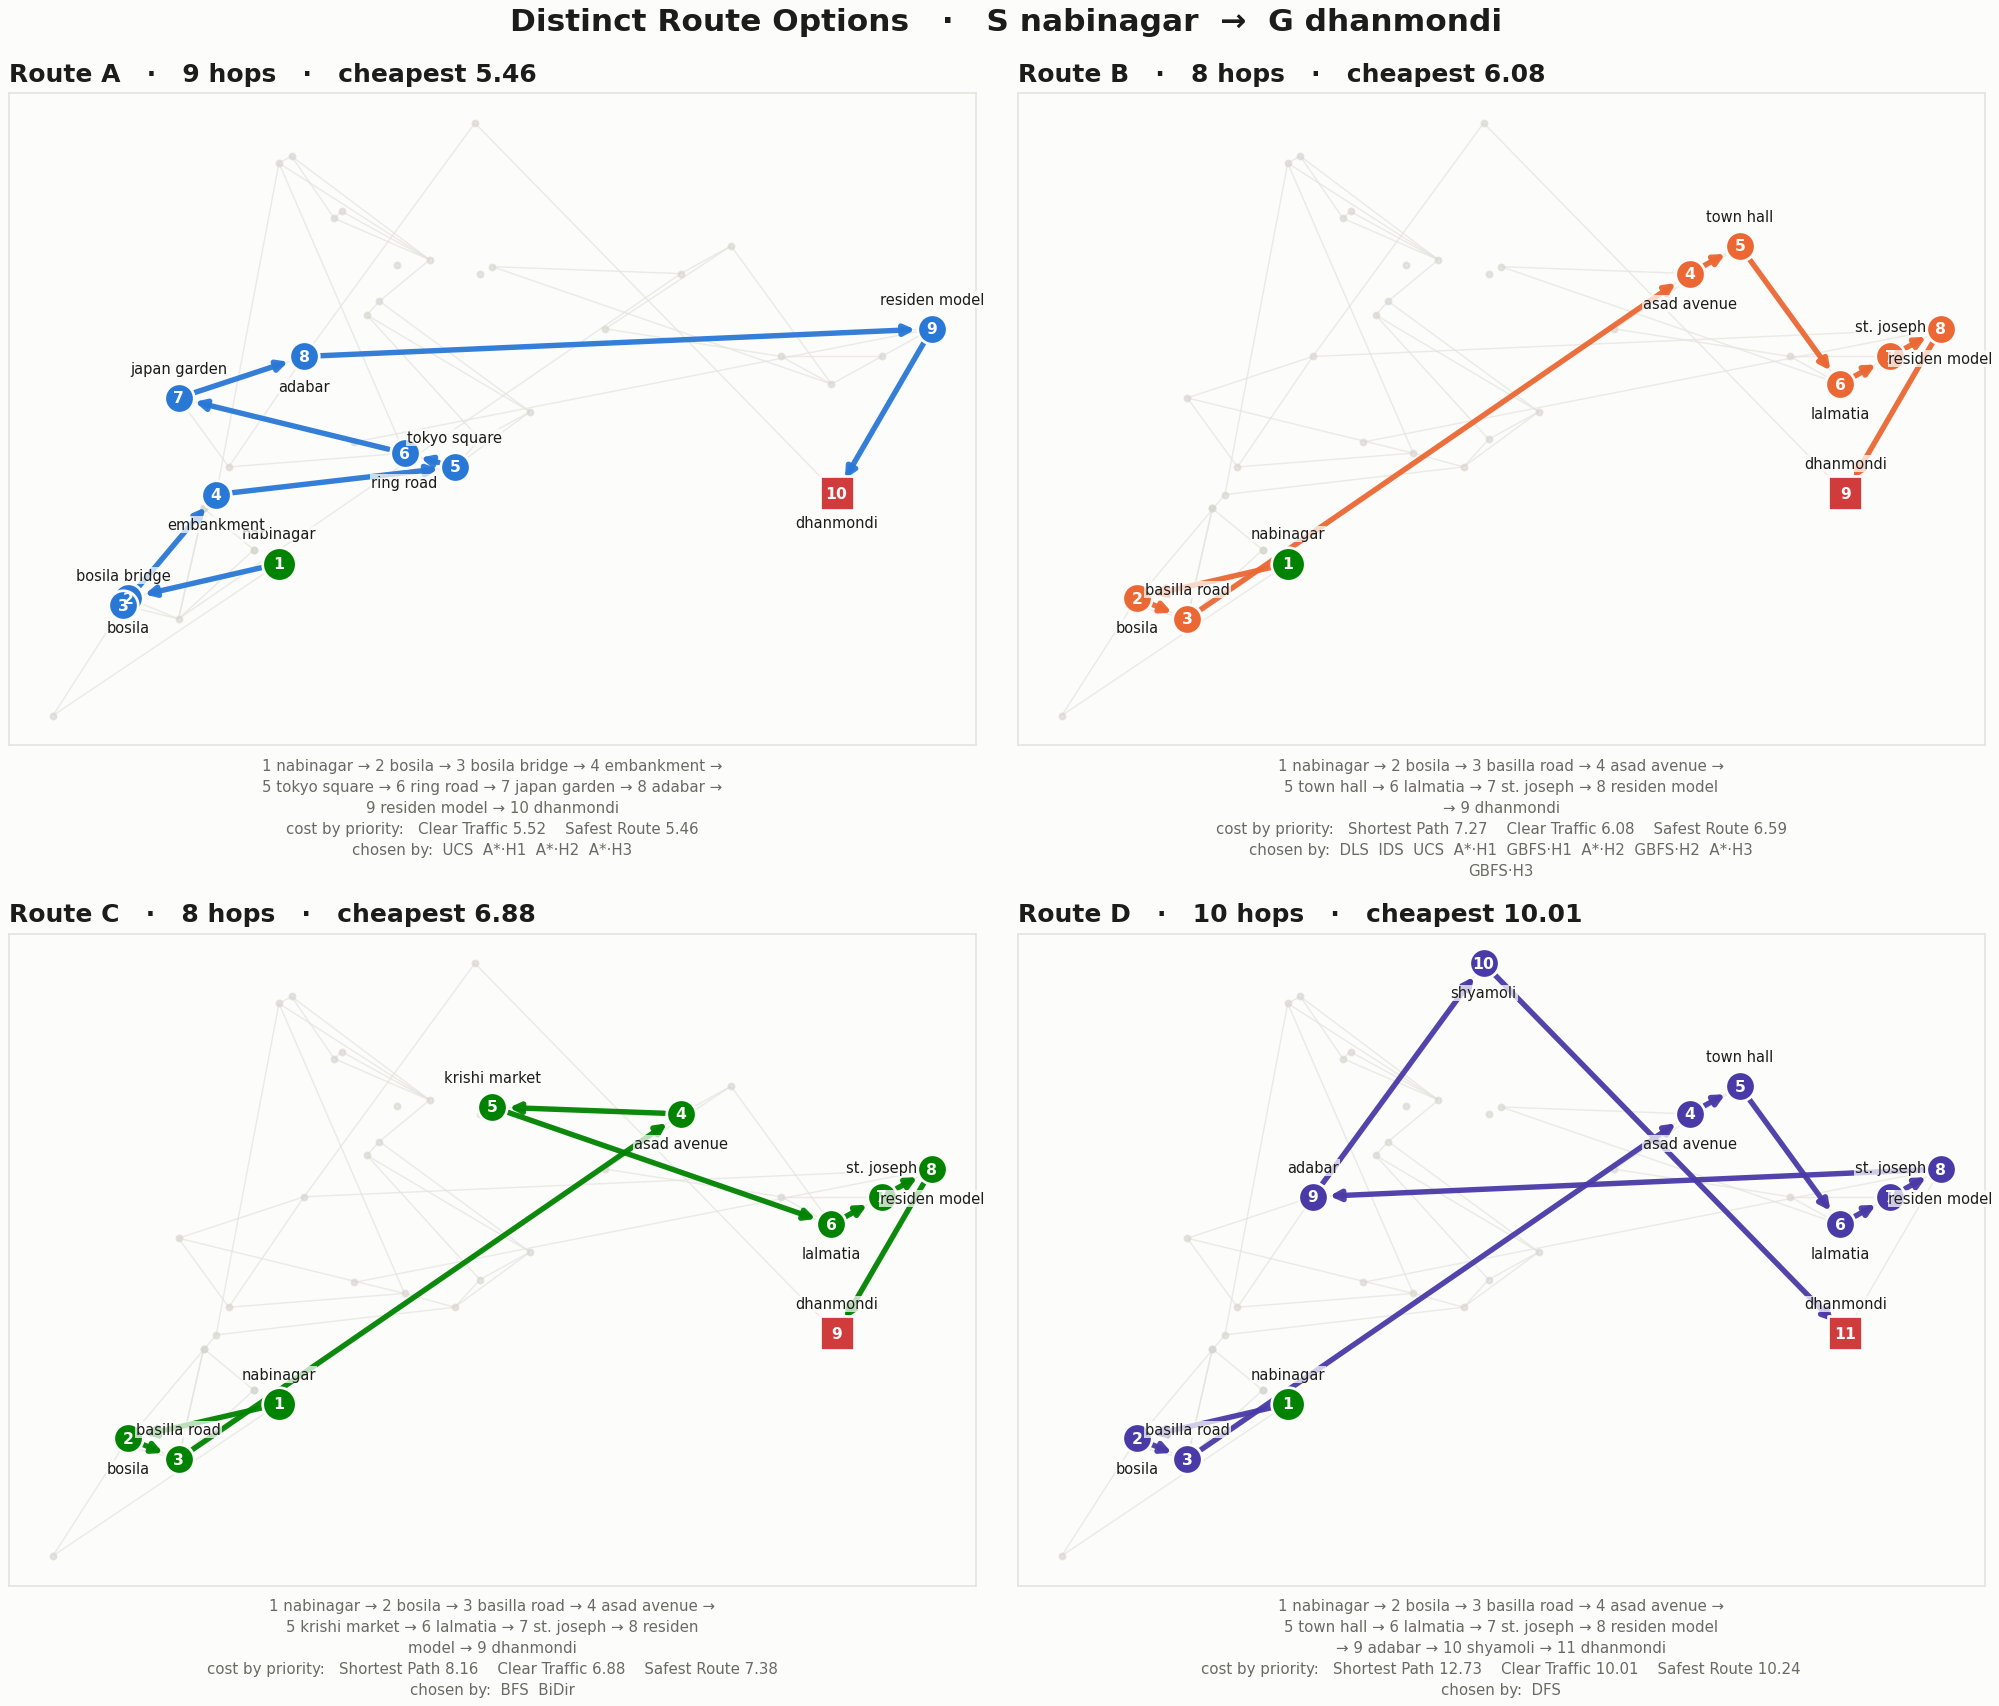
\includegraphics[width=0.72\textwidth]{cs1_routes.png}
\caption{CS-1: the distinct origin-to-destination routes the twelve strategies
actually select, drawn on the corridor and lettered by ascending cost. Cost-based
optimal search follows the genuinely cheapest route for each priority, whereas
depth-first and greedy search commit to longer or heuristically-tempting
alternatives. Visualizing the returned \emph{paths}---not just the metrics---makes
concrete why an admissible heuristic changes which road is chosen.}
\label{fig:cs1routes}
\end{figure}

\begin{figure}[tp]
\centering
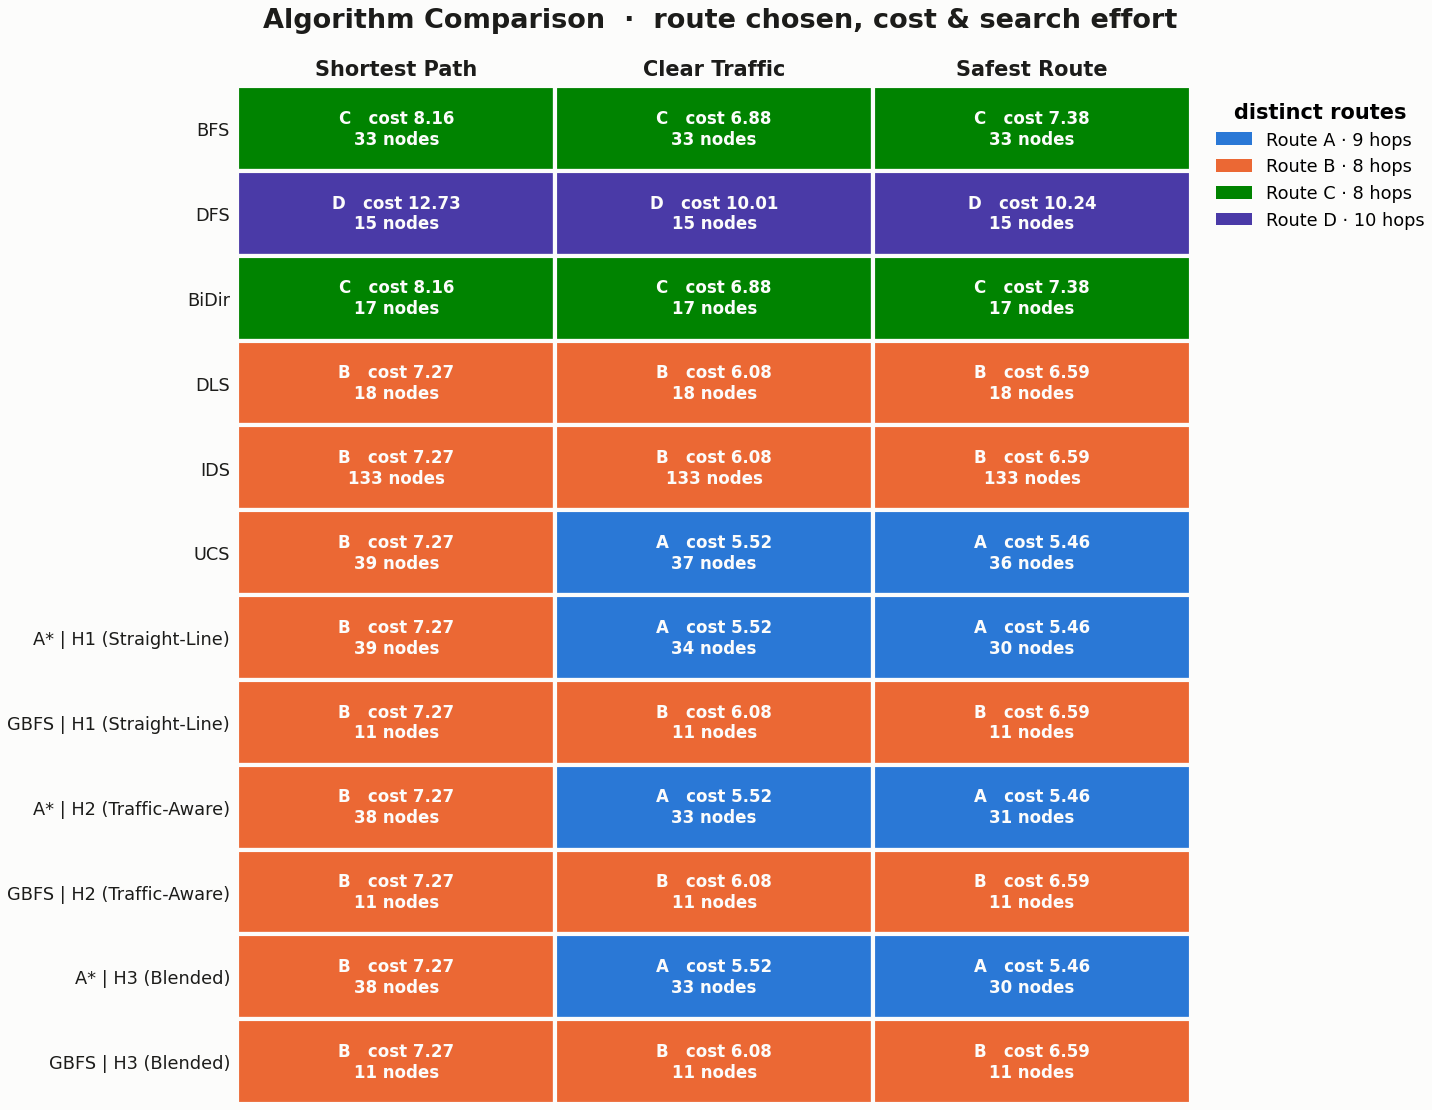
\includegraphics[width=0.80\textwidth]{cs1_matrix.png}
\caption{CS-1: which route each of the $12$ strategies selects under each of the
three priorities, annotated with path cost and nodes expanded. Cost-based
optimal search (UCS/A$^\star$) migrates to the genuinely cheapest route as the
priority shifts toward traffic and safety; heuristic-only and blind methods do
not.}
\label{fig:cs1matrix}
\end{figure}

\begin{figure}[tp]
\centering
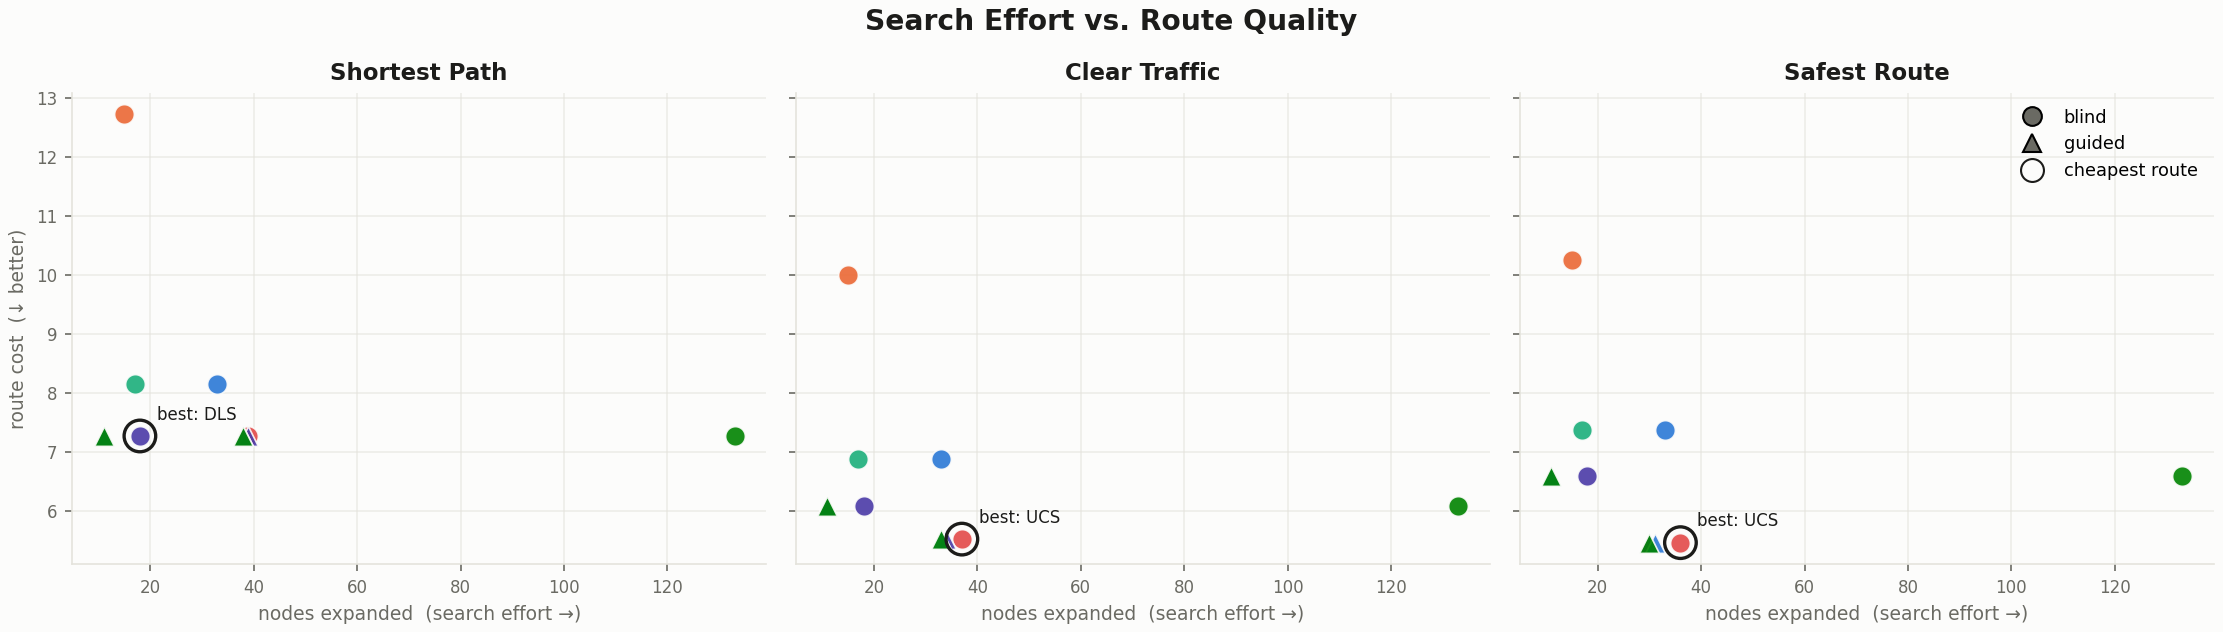
\includegraphics[width=\textwidth]{cs1_effort.png}
\caption{CS-1: search effort (nodes expanded) versus solution cost. Informed
methods (triangles) dominate the lower-left efficient region; A$^\star$ reaches
optimal cost at a fraction of the blind-search effort.}
\label{fig:cs1effort}
\end{figure}

\paragraph{Structural lesson.}
When the state space is small and fully known and a good admissible heuristic
exists, \emph{informed exact search (A$^\star$) is the right tool}: it keeps
optimality while paying the least for it. Greedy search is justified only when
speed strictly dominates quality.

%=======================================================================
\section{Case Study 2: Fuel Rationing as Constraint Satisfaction}
%=======================================================================
\subsection{Problem scenario}
During an acute fuel shortage, a city authority must ration supply across the
Gulshan--Banani corridor of Dhaka. Every stranded vehicle needs an
\emph{operating profile}---how fast it may drive, how much fuel it is allotted,
when it may refuel and at which station---and these choices cannot be made
independently: filling stations have limited bays and finite stock, whole fleets
must not all descend on the same pump at once, ambulances must be served before
ordinary cars, and the city's total daily ration is capped. The goal is not to
optimize a number but to find \emph{any} assignment that satisfies every rule
simultaneously---a pure feasibility problem over a combinatorial space. This is
the natural home of constraint satisfaction.

\subsection{Formal model}
We model the situation as a CSP $\langle X, D, C\rangle$. Each \textbf{variable}
$x_i \in X$ is a vehicle stranded in the corridor. The common \textbf{domain} $D$
is the set of $4$-tuples $(\text{speed},\text{quota},\text{slot},\text{station})$,
i.e.\ every legal operating profile, with
$|D| = 6\times4\times5\times6 = 720$ raw values per vehicle. The
\textbf{constraints} $C$ are $11$ rules of three kinds:
\begin{itemize}[leftmargin=1.4em,itemsep=0pt]
\item \textbf{Five unary (per-vehicle) constraints}, C1--C5: speed legality (obey
the road and vehicle limits), quota bounds (between the daily minimum need and the
tank capacity), reachability (the reserve fuel must actually get the vehicle to
its chosen station at its chosen speed), a traffic-window cap during rush hours,
and an emergency-window rule (ambulances/fire refuel in the earliest slots).
\item \textbf{Three binary (pairwise) constraints}, C6--C8: speed harmonization
(vehicles sharing a road corridor must not differ wildly in speed), fleet
dispersion (one fleet may not stack the same station-and-slot), and emergency
precedence (an emergency vehicle refuels before an ordinary one at a shared
station). These induce the \emph{constraint graph}.
\item \textbf{Three global ($n$-ary) constraints}, C9--C11: per-slot bay capacity,
per-station fuel stock, and the city-wide ration budget.
\end{itemize}
A solution is a total assignment $A:X\to D$ satisfying all $11$ constraints at
once; the raw search space is $720^{n}$ (about $10^{57}$ at $n{=}20$). A separate
verifier re-checks every constraint on the returned solution, decoupling
correctness from the solver.

\subsection{Algorithms}
We solve the CSP with backtracking search and progressively add: the
minimum-remaining-values variable heuristic with a degree tie-break (MRV), the
least-constraining-value ordering (LCV), forward checking (FC) and arc
consistency (AC-3). As a contrasting family we also run min-conflicts local
search with random restarts. Node consistency prunes the domain up front; a
separate verifier re-checks all $11$ constraints on the returned solution.

\subsection{Results}
Node consistency alone shrinks the $720$-value domain to a mean of $255$ surviving
values (min $30$, max $504$). On the $20$-vehicle visualization instance the full
configuration solves in $0.147$\,s with only $21$ search nodes, $0$ backtracks and
$838$ values pruned by inference; the independent verifier confirms all $11$
constraints hold ($120$\,L rationed against a $156$\,L city budget).

The decisive result is the \emph{phase transition}
(Table~\ref{tab:cs2}). We scale the instance toward the point where the number of
vehicles equals the total number of station-slots (a fully saturated,
$100\%$-load instance). Below saturation every configuration solves trivially. At
saturation ($n{=}40$) the behaviour splits: plain backtracking exhausts its
$2500$-node budget after $2461$ backtracks and \emph{fails}, whereas simply adding
the MRV heuristic solves the identical instance in $41$ nodes with \emph{zero}
backtracking. Inference (FC, AC-3) solves it too, at slightly higher constant
cost per node.

\begin{table}[tb]
\centering
\caption{CS-2 phase transition at $100\%$ load. ``nd'' $=$ search nodes,
``bt'' $=$ backtracks. At the saturated instance ($n{=}40$) plain backtracking
walls; MRV crosses it in $41$ nodes with no backtracking.}
\label{tab:cs2}
\small
\renewcommand{\arraystretch}{1.15}
\fitcol{%
\begin{tabular}{@{}l l r r l@{}}
\toprule
$n$ & \textbf{Config} & \textbf{nd} & \textbf{bt} & \textbf{Result} \\
\midrule
30 & plain BT   & 31   & 0    & solved \\
30 & MRV        & 31   & 0    & solved \\
36 & plain BT   & 37   & 0    & solved \\
36 & MRV        & 37   & 0    & solved \\
\midrule
40 & plain BT   & 2500 & 2461 & \textbf{FAIL (budget)} \\
40 & MRV        & 41   & 0    & solved \\
40 & MRV+FC     & 41   & 0    & solved \\
40 & MRV+FC+AC-3 & 41  & 0    & solved \\
\bottomrule
\end{tabular}}
\end{table}

Across the scaling experiment the best configuration's runtime grows smoothly
from $0.017$\,s at $n{=}8$ to $0.944$\,s at $n{=}40$, while min-conflicts reaches
a satisfying assignment in $4$ to $50$ repair steps---an order-of-magnitude
cheaper than the systematic search near saturation, at the cost of completeness
guarantees. Figures~\ref{fig:cs2model} and~\ref{fig:cs2search} show the model
(domain pruning and constraint graph) and the search behaviour. Every returned
assignment is checked by an independent verifier that re-evaluates all $11$
constraints from the raw problem data rather than trusting the solver's internal
bookkeeping; all reported solutions pass, dispensing $120$\,L of the $156$\,L
city budget.

\begin{figure}[tp]
\centering
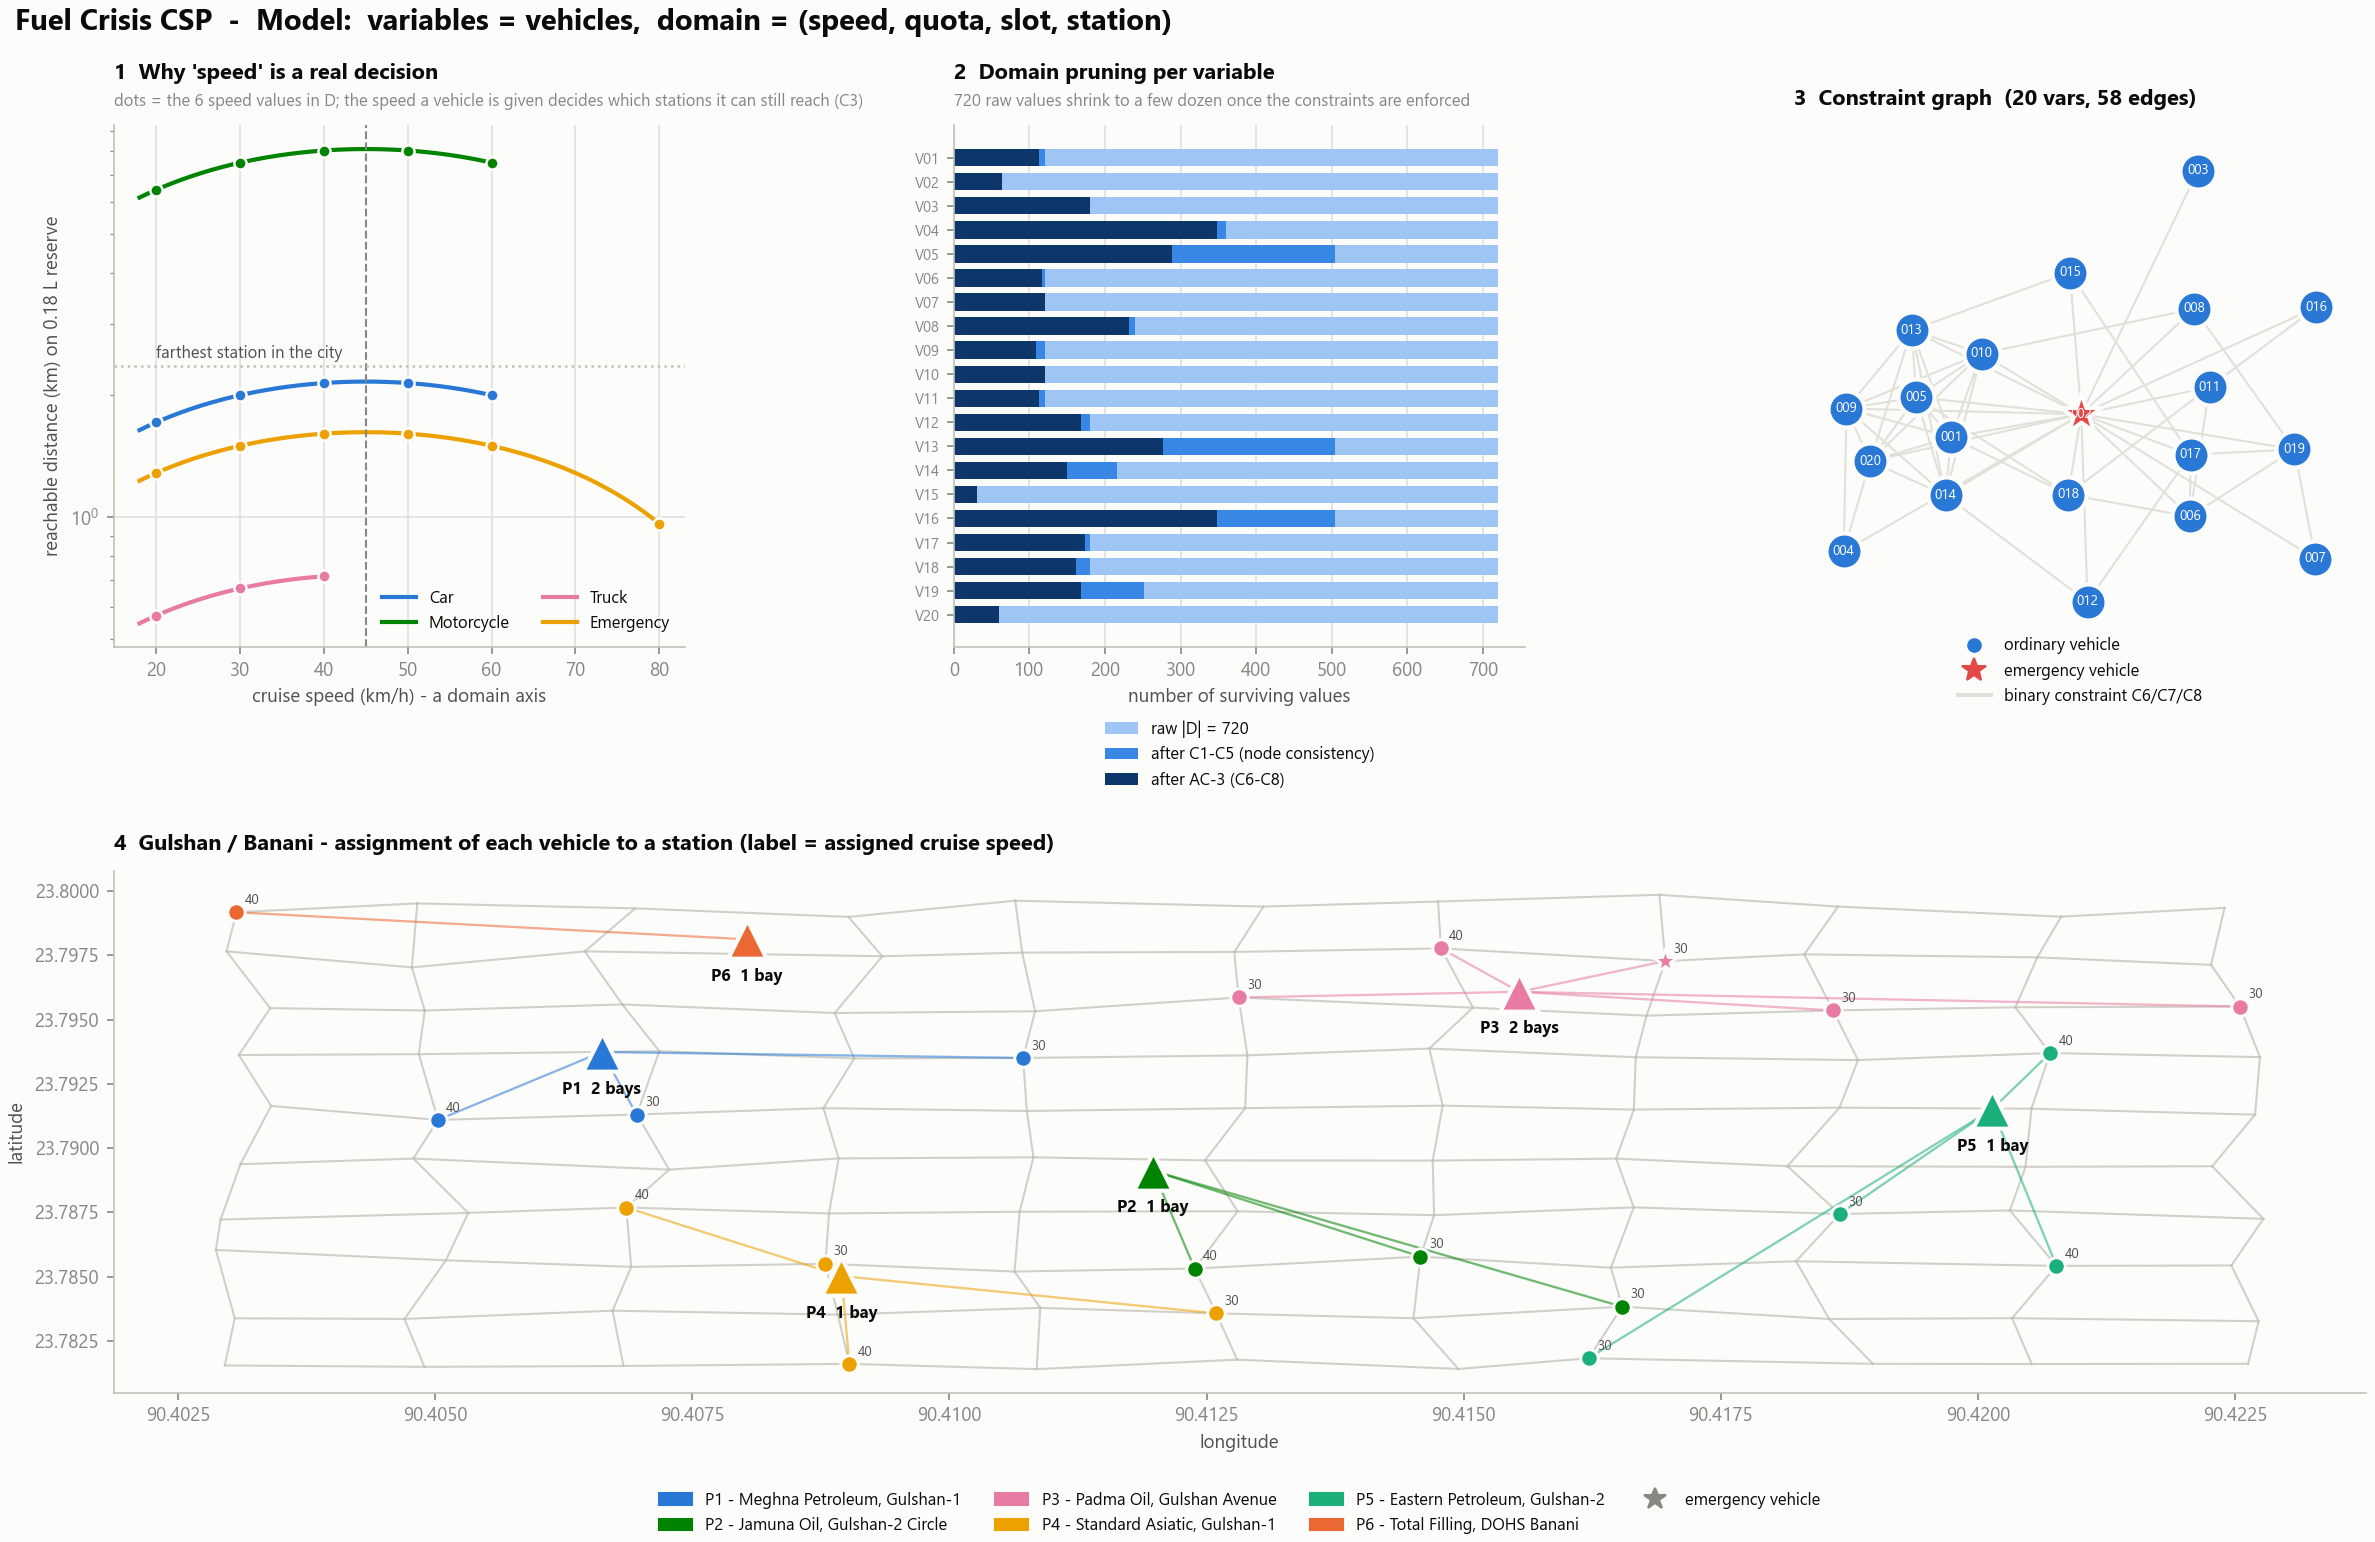
\includegraphics[width=0.85\textwidth]{cs2_model.png}
\caption{CS-2 model: fuel-economy-vs-speed motivation for the speed variable,
per-variable domain pruning ($720 \to$ tens of values), the binary constraint
graph, and the city map of stations and vehicles.}
\label{fig:cs2model}
\end{figure}

\begin{figure}[tp]
\centering
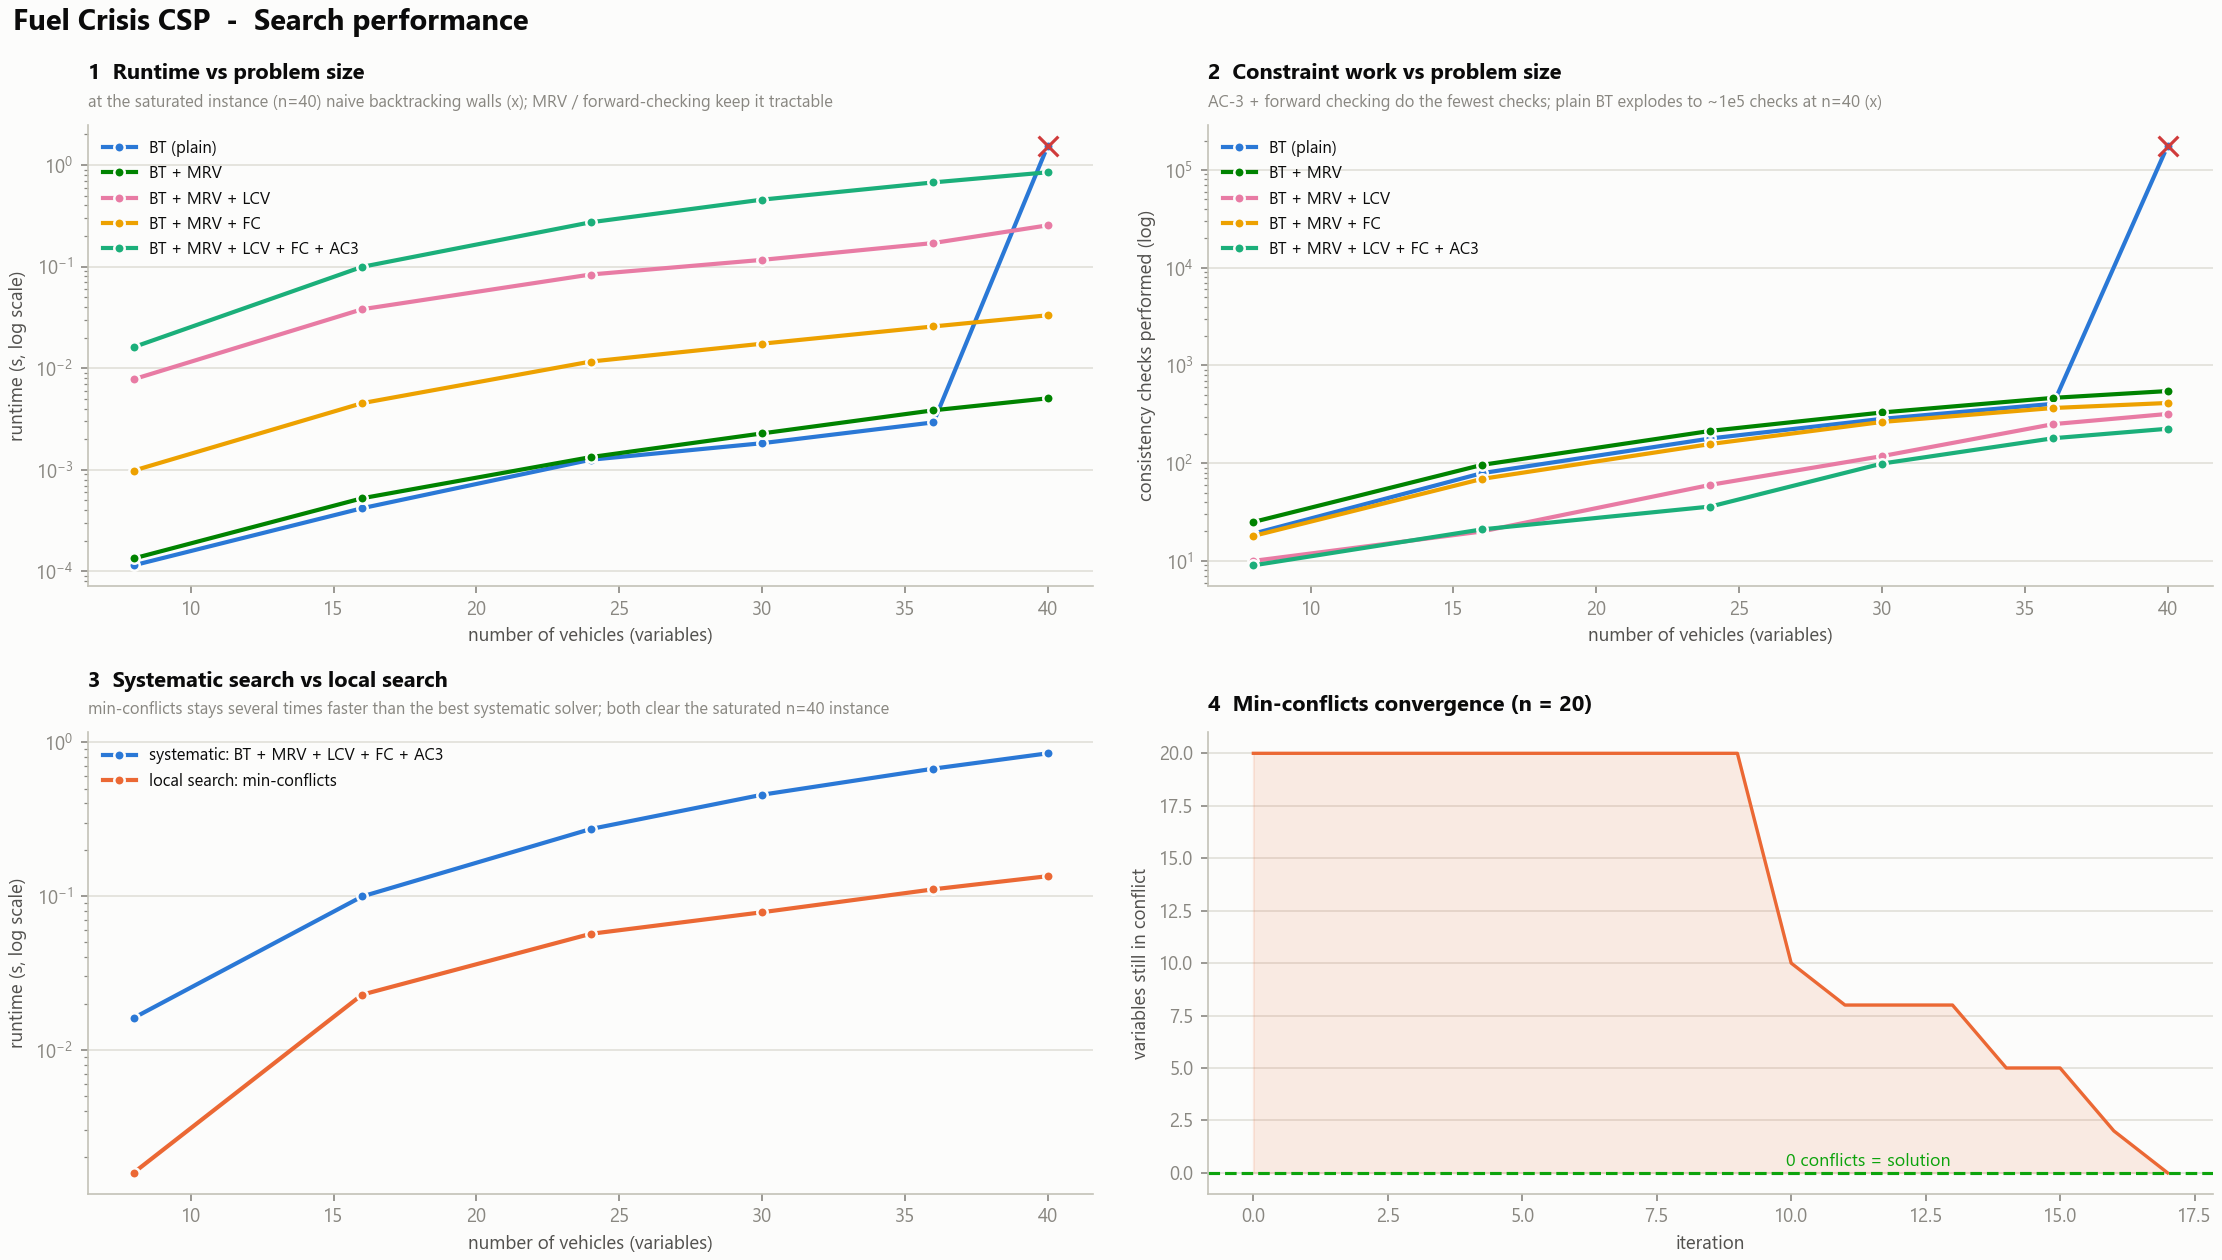
\includegraphics[width=0.86\textwidth]{cs2_search.png}
\caption{CS-2 search performance: runtime and consistency-check work versus
problem size for five backtracking configurations, systematic-vs-local search,
and the min-conflicts convergence trace. Naive backtracking explodes at the
saturated instance while heuristic/inference variants stay tractable.}
\label{fig:cs2search}
\end{figure}

\paragraph{Structural lesson.}
When the problem is combinatorial feasibility under hard constraints, the raw
search space is astronomically large but \emph{structured}. The right tools are
not brute force but \emph{constraint inference and ordering heuristics}: MRV alone
converts an unsolvable saturated instance into a $41$-node walk. Local search
(min-conflicts) is the pragmatic choice when speed matters more than a
completeness guarantee.

%=======================================================================
\section{Case Study 3: Smart Agriculture---Optimization and Learning}
%=======================================================================
\subsection{Problem scenario}
Declining natural-pollinator populations motivate \emph{robotic pollination}: a
fleet of small autonomous drones that fly through a greenhouse and pollinate
flowers. We model a $100\times100$\,m greenhouse containing $400$ flowers grown in
six natural clusters (planting beds), $5$ pollination robots that depart from
fixed depots along one edge, $3$ charging stations, and $25$ static obstacles
(support posts, water channels, equipment). Each robot has a finite battery that
caps its flying range, consumes energy per metre flown, and spends a fixed time
pollinating each flower. Running such a fleet well raises \emph{two structurally
different questions that must be answered in sequence}, which is why CS-3 tests
the paper's thesis twice (Figure~\ref{fig:pipeline}):
\begin{itemize}[leftmargin=1.4em,itemsep=1pt]
\item \textbf{Allocation (``who does what?'').} \emph{Which} robot should be
responsible for \emph{which} flowers, so that all flowers are covered with the
least total travel, energy and time, and no robot is overloaded? This is a static,
global combinatorial-optimization problem.
\item \textbf{Navigation (``how does it move?'').} Once a robot owns a set of
flowers, \emph{how} should it actually move---cell by cell, motor slip and
all---to visit them and return to a charger? This is a dynamic, per-robot
sequential-control problem under uncertainty.
\end{itemize}
The two are deliberately decomposed: Phase~1 outputs an assignment (exported as a
CSV), and Phase~2 consumes it as fixed input. Solving each with the family that
fits its structure---rather than forcing one method to do both---is itself an
instance of the paper's argument.

\begin{figure}[tp]
\centering
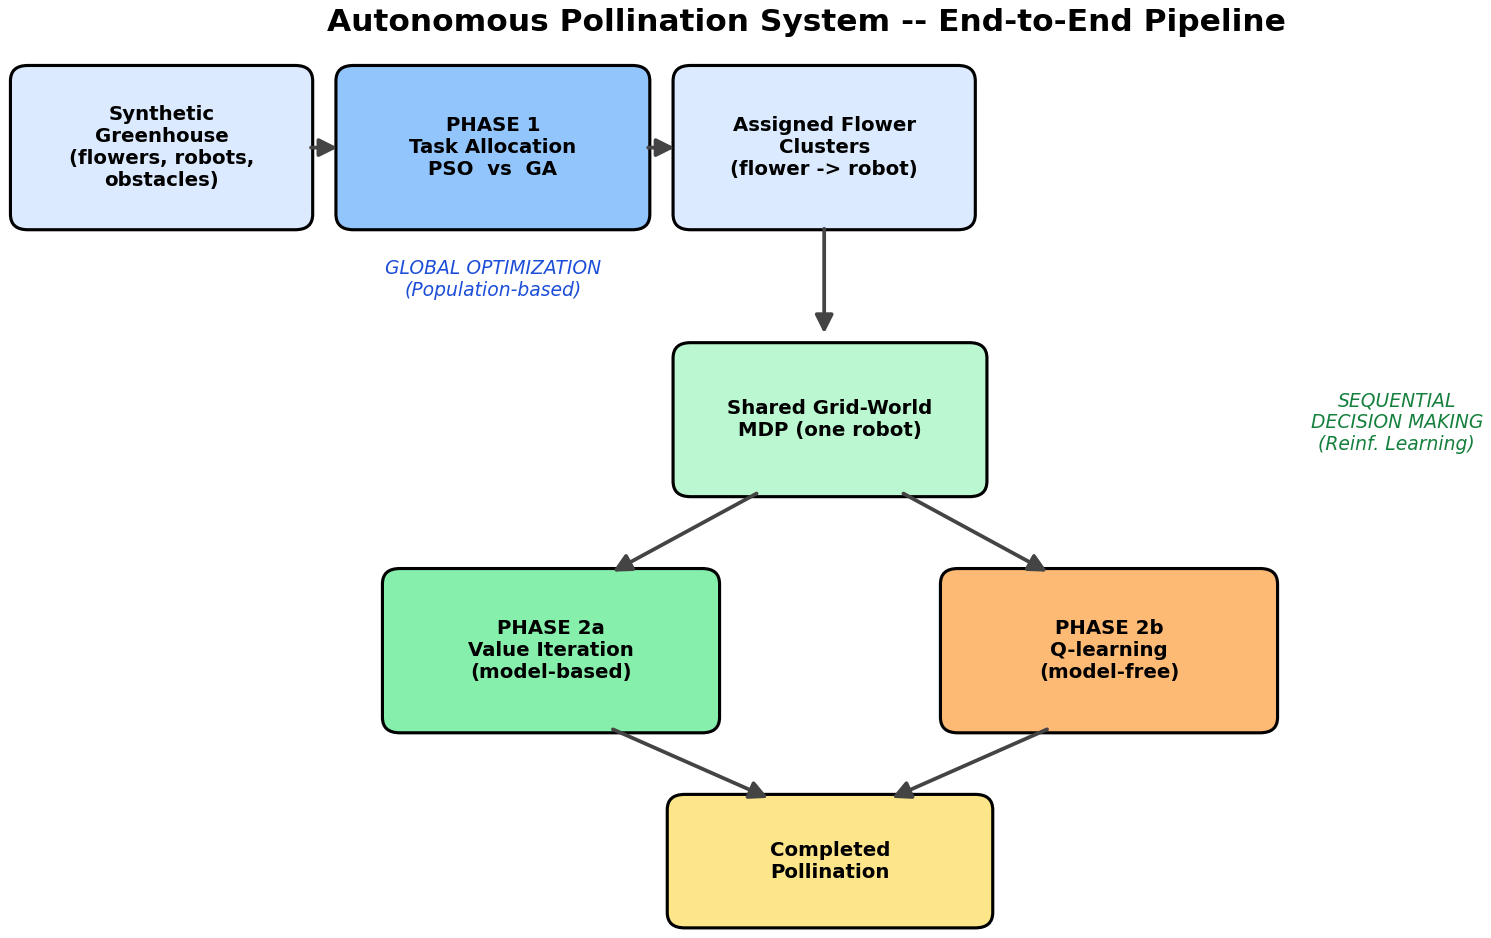
\includegraphics[width=0.66\textwidth]{fig_pipeline.png}
\caption{The smart-agriculture pipeline (CS-3). A combinatorial allocation phase
(metaheuristics) feeds a stochastic navigation phase (dynamic programming /
reinforcement learning). The clean CSV interface between phases lets each be
validated independently.}
\label{fig:pipeline}
\end{figure}

\subsection{Phase 1: task allocation (metaheuristics)}
\paragraph{Formulation.}
The decision is a map $a:\{1,\dots,400\}\to\{1,\dots,5\}$ assigning every flower to
a robot, giving a space of $5^{400}$ candidate assignments---more than the number
of atoms in the observable universe. The assignment is scored by a single fitness
(to be minimized) that blends \emph{six competing objectives}, each normalized to
be of comparable magnitude:
\begin{enumerate}[leftmargin=1.5em,itemsep=0pt]
\item \textbf{Coverage} --- fraction of flowers actually reachable within battery
range (strongly rewarded; every flower should be served);
\item \textbf{Total travel distance} --- summed over all robots' routes;
\item \textbf{Energy} --- battery units consumed (proportional to distance);
\item \textbf{Completion time} --- the makespan, i.e.\ the slowest robot's finish
time, since robots fly in parallel;
\item \textbf{Workload imbalance} --- the standard deviation of flowers-per-robot
(a fair split is preferred);
\item \textbf{Robot under-utilization} --- penalizes leaving robots idle.
\end{enumerate}
Each robot's route cost is estimated with a fast greedy nearest-neighbour tour.
This is an \emph{upper bound} on the optimal tour, not an admissible
(underestimating) heuristic in the A$^\star$ sense; it serves as a consistent,
cheap surrogate that ranks allocations without solving the routing problem, which
belongs to Phase~2 rather than the allocator. The objective is therefore \emph{discrete} (a flower goes to robot~2
or robot~3, never $2.5$), \emph{non-linear and coupled} (a robot's cost depends on
the whole set of flowers it receives---a routing sub-problem), and
\emph{multi-objective}. This combination---huge, discrete, non-differentiable,
multi-objective---is the textbook signature of an NP-hard problem for which
population-based metaheuristics, not exact search or gradient methods, are the
appropriate family.

\paragraph{Algorithms.}
Both a particle swarm optimizer (continuous encoding, floored to robot indices)
and a genetic algorithm (native discrete encoding: tournament selection, uniform
crossover, random-reset mutation, elitism, and a fraction of the population seeded
with a nearest-depot heuristic) optimize the \emph{identical} fitness on the
\emph{identical} greenhouse.

\paragraph{Results.}
Table~\ref{tab:cs3alloc} shows the genetic algorithm dominating on every headline
metric, and---because we now average over $10$ seeds on the fixed greenhouse---the
margin is demonstrably not luck: the GA--PSO fitness gap ($\approx0.17$) is more
than three times the two seed spreads \emph{added together} ($\pm0.02$ and
$\pm0.03$), and over five times either one alone. Its native discrete
encoding, together with heuristic seeding that injects spatial structure, reaches a
lower (better) fitness ($1.43$ vs.\ PSO's $1.60$), a shorter
total distance ($2203$\,m vs.\ $2450$\,m), and---most strikingly---a far more even
\emph{and} more consistent workload (per-robot count std $1.27{\pm}0.47$ vs.\
$2.86{\pm}1.10$: PSO is both worse and more variable), for roughly $1.7\times$
PSO's wall-clock time. Continuous PSO's known weakness in
very high dimensions ($400$ here) shows: its encoding has no built-in notion that
spatially close flowers should share a robot, so it must discover that structure
from scratch, and within the same budget it does not.
Figures~\ref{fig:cs3psoga} and~\ref{fig:cs3gamap} present the
comparison and the evolved allocation map.

\begin{table}[tb]
\centering
\caption{CS-3 Phase 1: task allocation ($400$ flowers, $5$ robots). Lower fitness
and workload-std are better. Both optimizers are reported as mean$\,\pm\,$std
over the same $10$ seeds on the fixed greenhouse; times are representative
wall-clock. The GA's advantage exceeds the seed spread on every metric.}
\label{tab:cs3alloc}
\small
\renewcommand{\arraystretch}{1.2}
\fitcol{%
\begin{tabular}{@{}l r r r r@{}}
\toprule
\textbf{Method} & \textbf{Fitness} & \textbf{Dist.\ (m)} & \textbf{Load std} & \textbf{Time (s)} \\
\midrule
PSO    & $1.600\,{\scriptstyle\pm.032}$ & $2450\,{\scriptstyle\pm49}$ & $2.86\,{\scriptstyle\pm1.10}$ & $\approx$10.6 \\
GA     & $\mathbf{1.434}\,{\scriptstyle\pm.020}$ & $\mathbf{2203}\,{\scriptstyle\pm40}$ & $\mathbf{1.27}\,{\scriptstyle\pm.47}$ & $\approx$18.4 \\
\bottomrule
\end{tabular}}
\end{table}

\begin{figure}[tp]
\centering
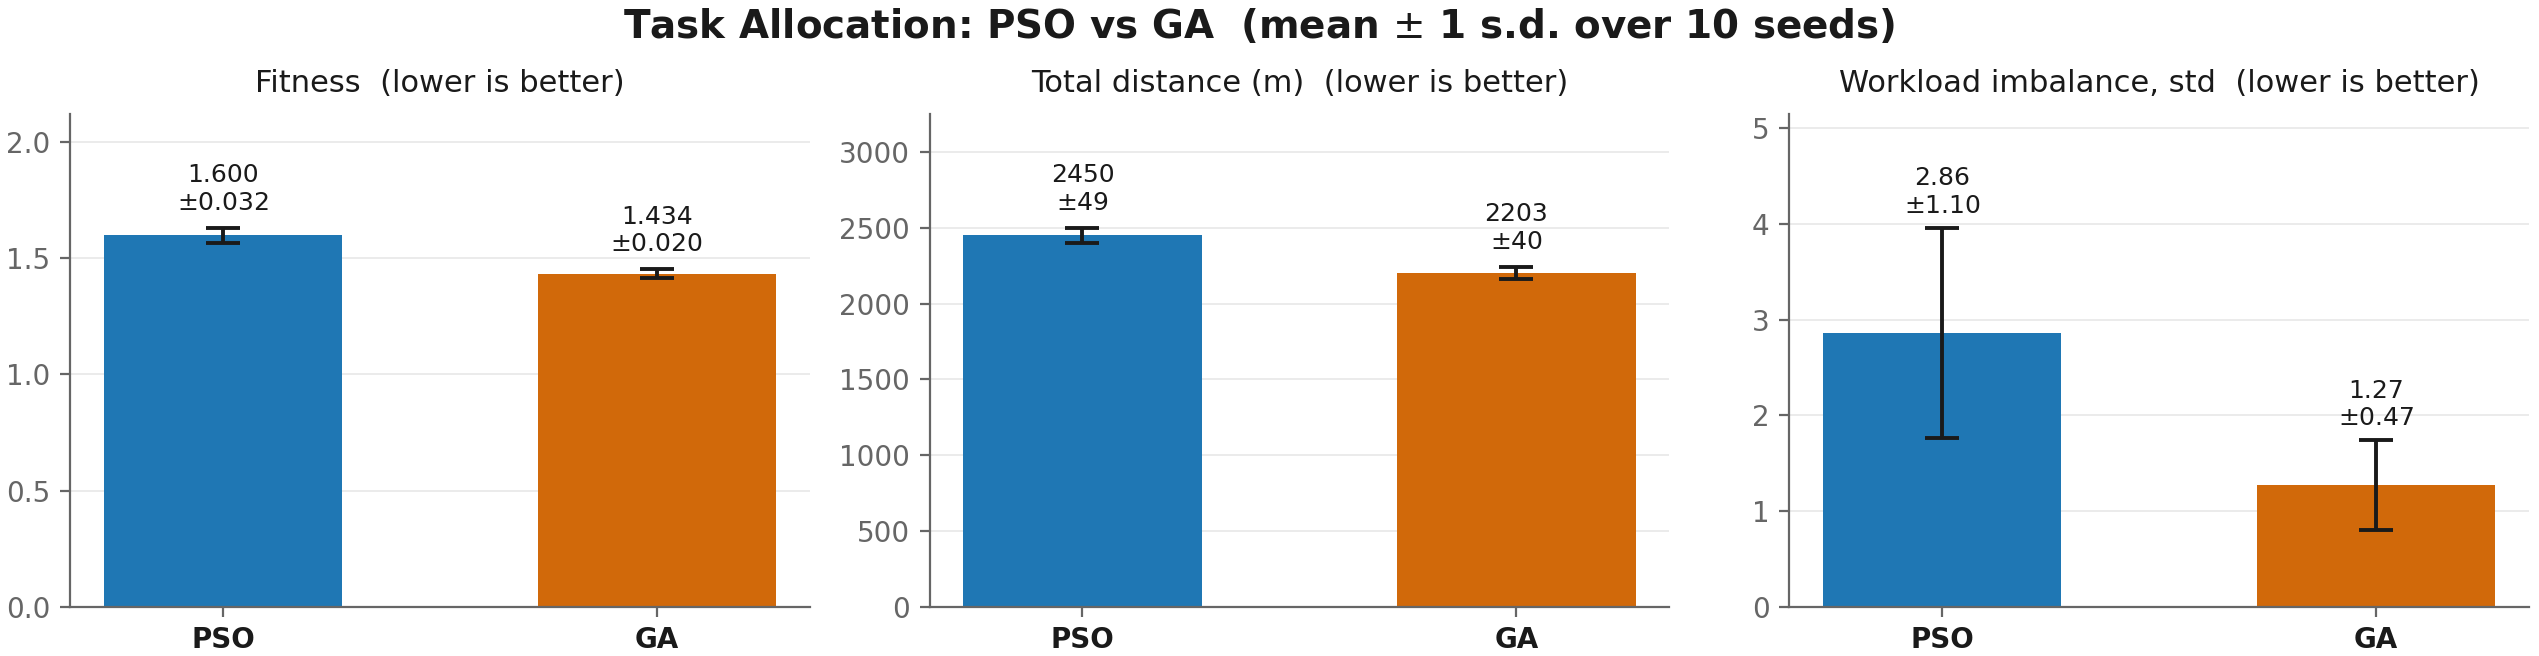
\includegraphics[width=\textwidth]{cs3_pso_vs_ga.png}
\caption{CS-3 Phase 1: PSO vs.\ GA on the three reported allocation metrics,
mean $\pm$ $1$ s.d.\ over the same $10$ seeds as Table~\ref{tab:cs3alloc}. The
GA is better on all three, and the gaps in fitness and distance are several
times the seed spread; workload balance is where the discrete encoding pays off
most, and it is also where PSO is least consistent.}
\label{fig:cs3psoga}
\end{figure}

% Square figure -- keep it to half the text width so it does not dominate the
% page in the single-column layout (a square at full width is ~16cm tall).
\begin{figure}[tb]
\centering
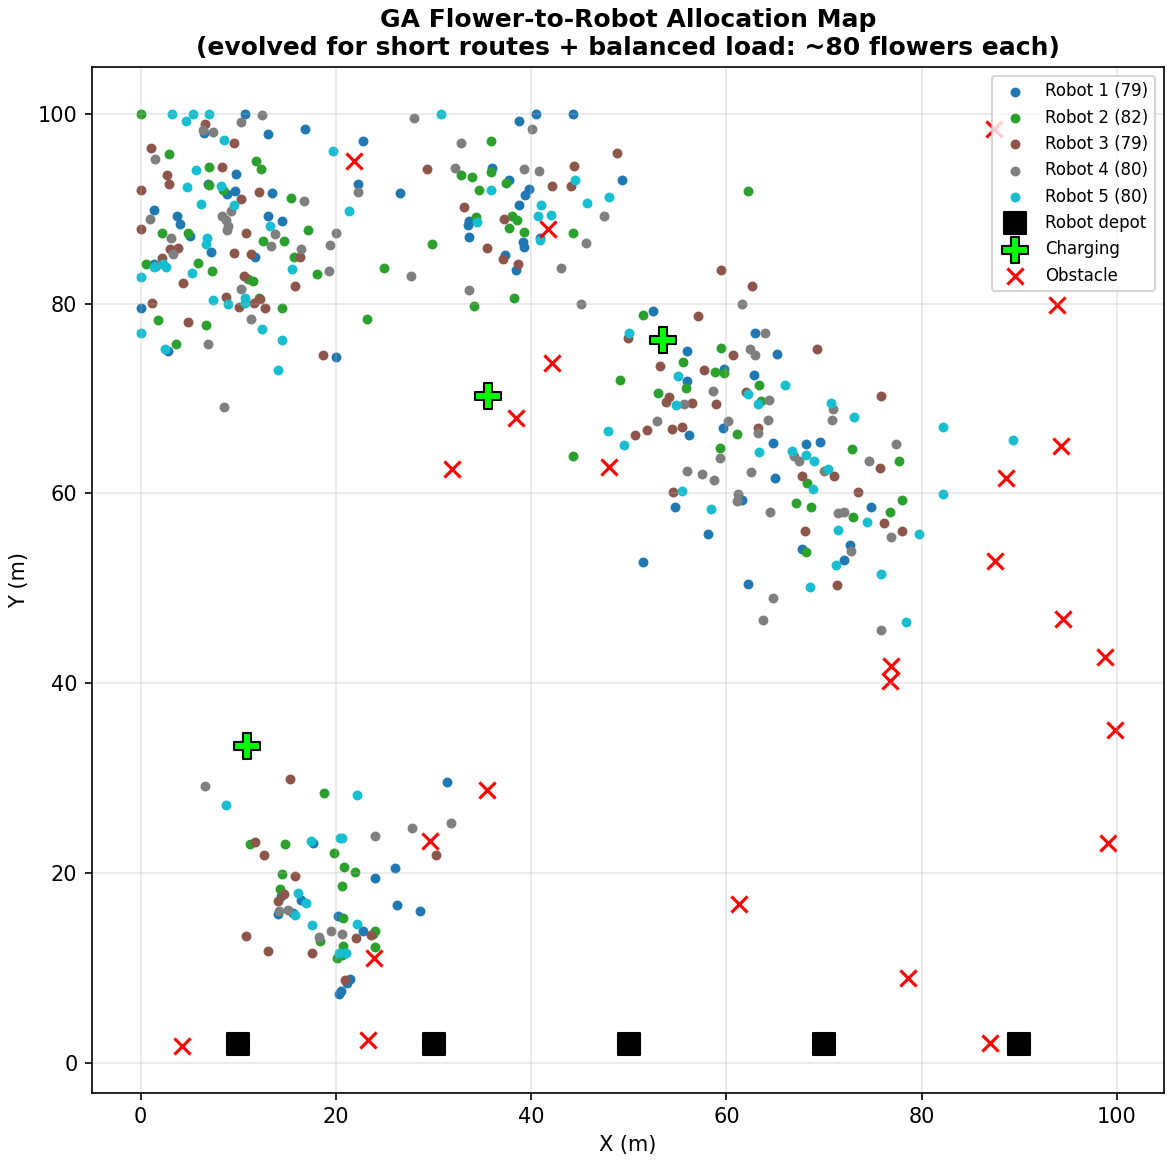
\includegraphics[width=0.5\textwidth]{cs3_ga_map.png}
\caption{CS-3 Phase 1: the genetic algorithm's evolved flower-to-robot allocation,
coloured by robot---spatially coherent clusters with roughly balanced load.}
\label{fig:cs3gamap}
\end{figure}

\subsection{Phase 2: navigation (value iteration vs.\ Q-learning)}
\paragraph{Formulation.}
We now zoom into a \emph{single} robot and the flowers Phase~1 gave it. The
continuous greenhouse is discretized into a $20\times20$ grid; obstacle,
charging and flower coordinates map to grid cells. The robot must visit all its
target flowers and then return to a charging station. Formally this is a
\textbf{Markov decision process} $\langle S,A,T,R,\gamma\rangle$:
\begin{itemize}[leftmargin=1.4em,itemsep=0pt]
\item \textbf{States $S$.} A cell $(r,c)$ \emph{augmented} with a
$k$-bit visited-mask recording which of the $k$ target flowers are already
pollinated. The mask is essential: an MDP state is memoryless, so without it the
robot could not know when the multi-flower mission is complete or avoid
re-visiting.
\item \textbf{Actions $A$.} Move \textsc{up}, \textsc{down}, \textsc{left} or
\textsc{right}.
\item \textbf{Transitions $T$ (stochastic).} Actuation is noisy: the intended move
succeeds with probability $0.8$, and with probability $0.1$ each the robot
\emph{slips} to one of the two perpendicular cells. A move into an obstacle or
wall leaves the robot in place. This uncertainty is precisely why a single fixed
plan is inadequate---one slip and a pre-computed path is off track.
\item \textbf{Rewards $R$ (shared identically by both algorithms).} Reaching an
un-pollinated flower $+10$; returning to a charger once all flowers are done
$+10$; each ordinary step $-0.1$ (time/battery); colliding with an obstacle/wall
$-5$. Rewards are \emph{delayed}: the large flower reward may arrive many steps
after the moves that earned it, so the method must propagate credit backward.
\end{itemize}
Three structural cues therefore define the problem---decisions are
\emph{sequential} (each move changes where the next begins), outcomes are
\emph{stochastic}, and reward is \emph{delayed}. This is exactly the setting for
which a \emph{policy} (an action for every state), not a fixed path, is required,
and hence for dynamic programming and reinforcement learning rather than the
shortest-path search of CS-1. The one variable we manipulate is whether the
transition model is \emph{known}: value iteration is given it; Q-learning is not.

\paragraph{Algorithms.}
Value iteration solves the Bellman optimality equations on the \emph{known} model;
Q-learning learns a policy from interaction alone on the \emph{same} environment
with no model. Both are evaluated under the same stochastic roll-out.

Two honest caveats attach to the ``single variable'' framing. First, the
comparison is \emph{not} perfectly controlled: value iteration discounts at
$\gamma{=}0.9$ and Q-learning at $\gamma{=}0.95$, inherited from each method's own
tuning, so the model/no-model contrast is confounded with a small difference in
discounting. Figure~\ref{fig:cs3sens} is the evidence that this does not drive the
result---value iteration's recovered path is $63$--$65$ steps across the whole
$\gamma$ sweep, and Q-learning's reward varies by only $4.2$ across
configurations that include $\gamma$---but a clean study would fix $\gamma$ for
both. Second, Q-learning's convergence guarantee~\cite{watkins1992} assumes every
state--action pair is visited infinitely often \emph{and} a Robbins--Monro
learning-rate schedule ($\sum\alpha_t=\infty$, $\sum\alpha_t^2<\infty$). We use a
constant $\alpha{=}0.15$ and floor exploration at $\varepsilon{=}0.05$, as is
standard in practice; this converges to a bounded neighbourhood of $Q^{\star}$
rather than to $Q^{\star}$ itself. The parity we report is therefore an empirical
finding, not a theoretical entitlement.

We must be precise about \emph{which} MDP each one solves, because they differ.
Q-learning learns over the full mask-augmented state space
($20\times20\times2^{k}\times4$ action values) described above. Value iteration is
instead applied to a \emph{decomposition}: it solves a single-goal MDP over the
$400$ cells whose goal set is ``any remaining flower'', re-planning after each
flower is collected, and finally over the charger set. This is the standard
sequential-replanning treatment and it keeps value iteration's state space small,
but it is optimal only \emph{per leg}: the visiting \emph{order} it induces is
nearest-remaining-first, which is a greedy heuristic for what is really a
travelling-salesman-style ordering problem. Value iteration should therefore be
read here as a strong, model-informed baseline rather than a certified optimum for
the whole mission---a caveat that makes Q-learning's parity on reward more
notable, not less, since Q-learning optimizes the undecomposed problem directly.

\paragraph{Results.}
Table~\ref{tab:cs3nav} is the cleanest illustration of the whole paper's thesis.
Averaged over $10$ slip-seeds, both methods reach a $\approx$$100\%$ success rate
and \emph{statistically indistinguishable} policy quality (mean reward
$59.07{\pm}0.42$ for Q-learning vs.\ $59.13{\pm}0.21$ for value iteration; a
Welch two-sample $t$-test on the $10$ seeds gives $t{=}0.41$, $\mathrm{df}{=}13.3$,
$p{=}0.69$, so the $0.06$-reward difference is not distinguishable from seed
noise. The step counts do differ modestly, $88.5$ vs.\ $84.1$). But value iteration,
handed the model, converges in $36$ Bellman sweeps and $0.05$\,s (deterministically,
with no seed variance), whereas Q-learning must \emph{discover} the same behaviour
over $2223{\pm}130$ episodes and $\sim$$9.2$\,s---about $176\times$ slower. The gap
is not a defect: it is the price of
model-freedom. In a real greenhouse whose obstacle map and slip probabilities are
unknown, value iteration \emph{cannot run at all}, while Q-learning still can.
Figure~\ref{fig:cs3conv} places the two convergence processes side by side; the
head-to-head metrics are in Table~\ref{tab:cs3nav}.

Aggregate reward alone cannot show \emph{how} the two agents behave, so
Figure~\ref{fig:cs3paths} draws one episode of each on the same grid, both
executed under the same actuator-slip model. The routes are visibly not
identical---nothing forces a learner to reproduce a particular optimal
trajectory when several are near-optimal---but they are behaviourally
equivalent: both visit every flower, both return to a charger, and they finish
within a few steps of one another ($97$ vs.\ $101$ in the episodes shown; $84.1$
vs.\ $88.5$ on average). This is the honest form of the claim that Q-learning
``recovers'' the policy: it recovers the \emph{competence}, not the exact
argmax in every cell.

Finally, Figure~\ref{fig:cs3sens} checks that neither result is an artefact of a
lucky hyperparameter choice. Value iteration's sweep count grows smoothly with
$\gamma$ and with a tighter residual threshold $\theta$ ($22$--$63$ sweeps across
the grid) while the recovered path length is essentially fixed at $63$--$65$
steps: the extra sweeps buy precision in $V$, not a different policy. Q-learning
is likewise stable, with all seven configurations landing within a $4.2$-reward
band and success rates of $0.99$--$1.00$; the weakest is the fastest
$\varepsilon$-decay ($0.998$), which is the expected signature of too little
exploration rather than a tuning accident.

\begin{table}[tb]
\centering
\caption{CS-3 Phase 2: navigation under stochastic actuation. Performance rows
are mean$\,\pm\,$std over $10$ slip-seeds; VI's \emph{computation} (convergence,
execution time) is deterministic and carries no seed variance. Q-learning
rediscovers value iteration's near-optimal policy from zero model knowledge, at
$\sim$$176\times$ the compute.}
\label{tab:cs3nav}
\small
\renewcommand{\arraystretch}{1.2}
\fitcol{%
\begin{tabular}{@{}l r r@{}}
\toprule
\textbf{Metric} & \textbf{Value Iteration} & \textbf{Q-learning} \\
\midrule
Success rate        & $\mathbf{1.000}\,{\scriptstyle\pm.000}$  & $0.999\,{\scriptstyle\pm.002}$ \\
Mean reward         & $59.13\,{\scriptstyle\pm.21}$ & $59.07\,{\scriptstyle\pm.42}$ \\
Mean steps          & $84.1\,{\scriptstyle\pm.5}$   & $88.5\,{\scriptstyle\pm1.7}$ \\
Convergence         & 36 sweeps (det.) & $2223\,{\scriptstyle\pm130}$ ep. \\
Execution time (s)  & \textbf{0.052} (det.) & $\approx$9.2 \\
Model required?     & \textbf{Yes} & \textbf{No} \\
\bottomrule
\end{tabular}}
\end{table}

\begin{figure}[tp]
\centering
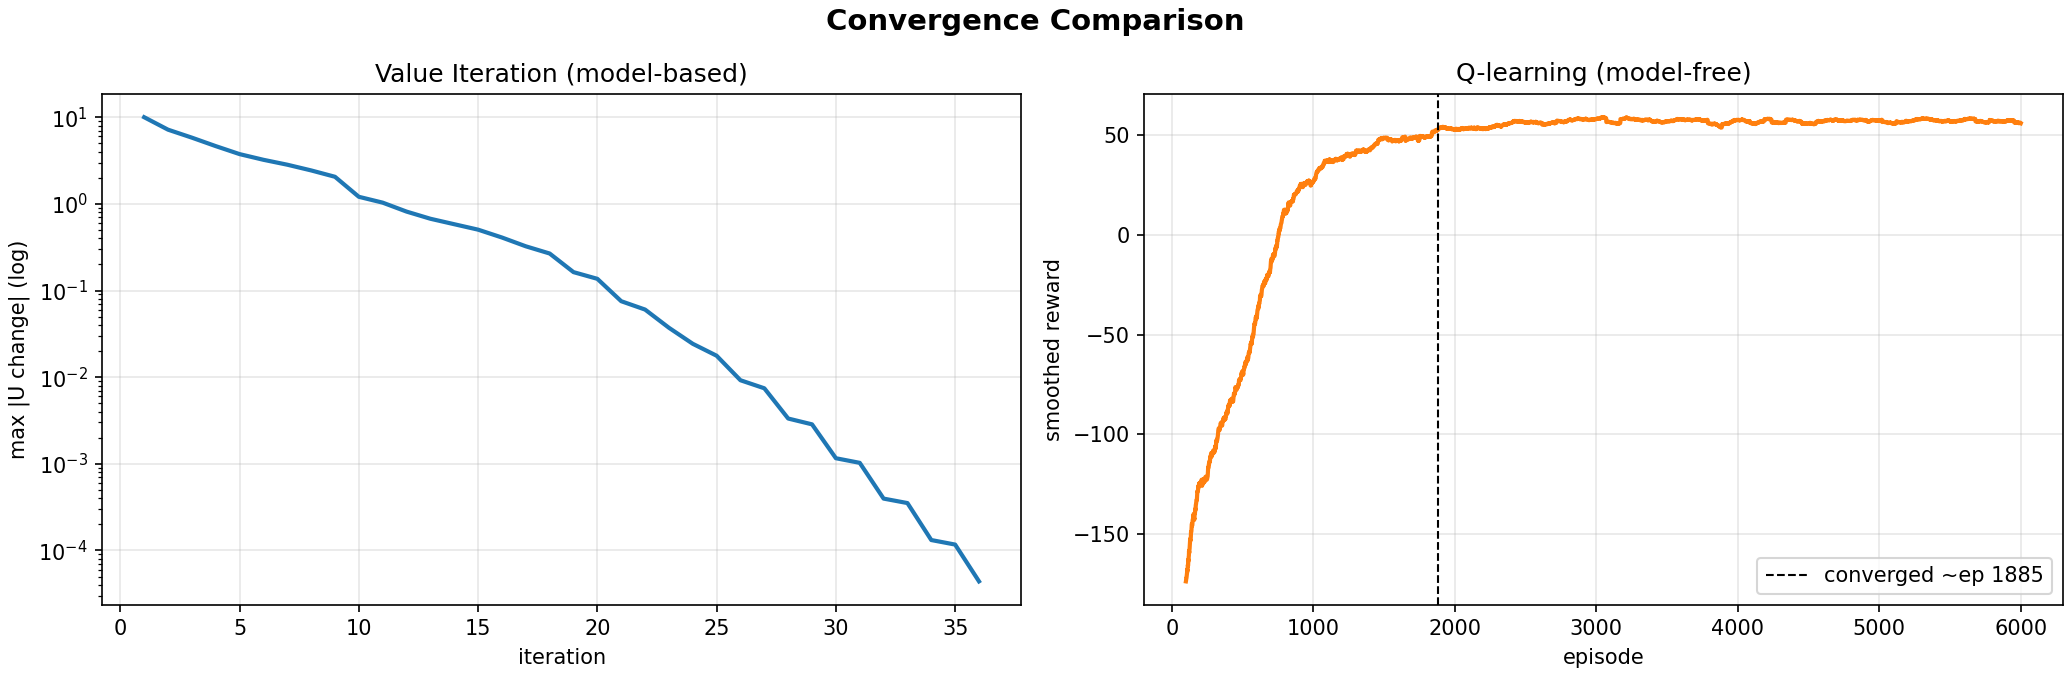
\includegraphics[width=\textwidth]{cs3_vi_ql_convergence.png}
\caption{CS-3 Phase 2: convergence processes. Value iteration (left) contracts the
Bellman residual in tens of sweeps; Q-learning (right) raises smoothed reward over
$\sim$$1885$ episodes in the run plotted here ($2223\,{\scriptstyle\pm130}$ over the
$10$ seeds)---different units, same destination.}
\label{fig:cs3conv}
\end{figure}

\begin{figure}[tp]
\centering
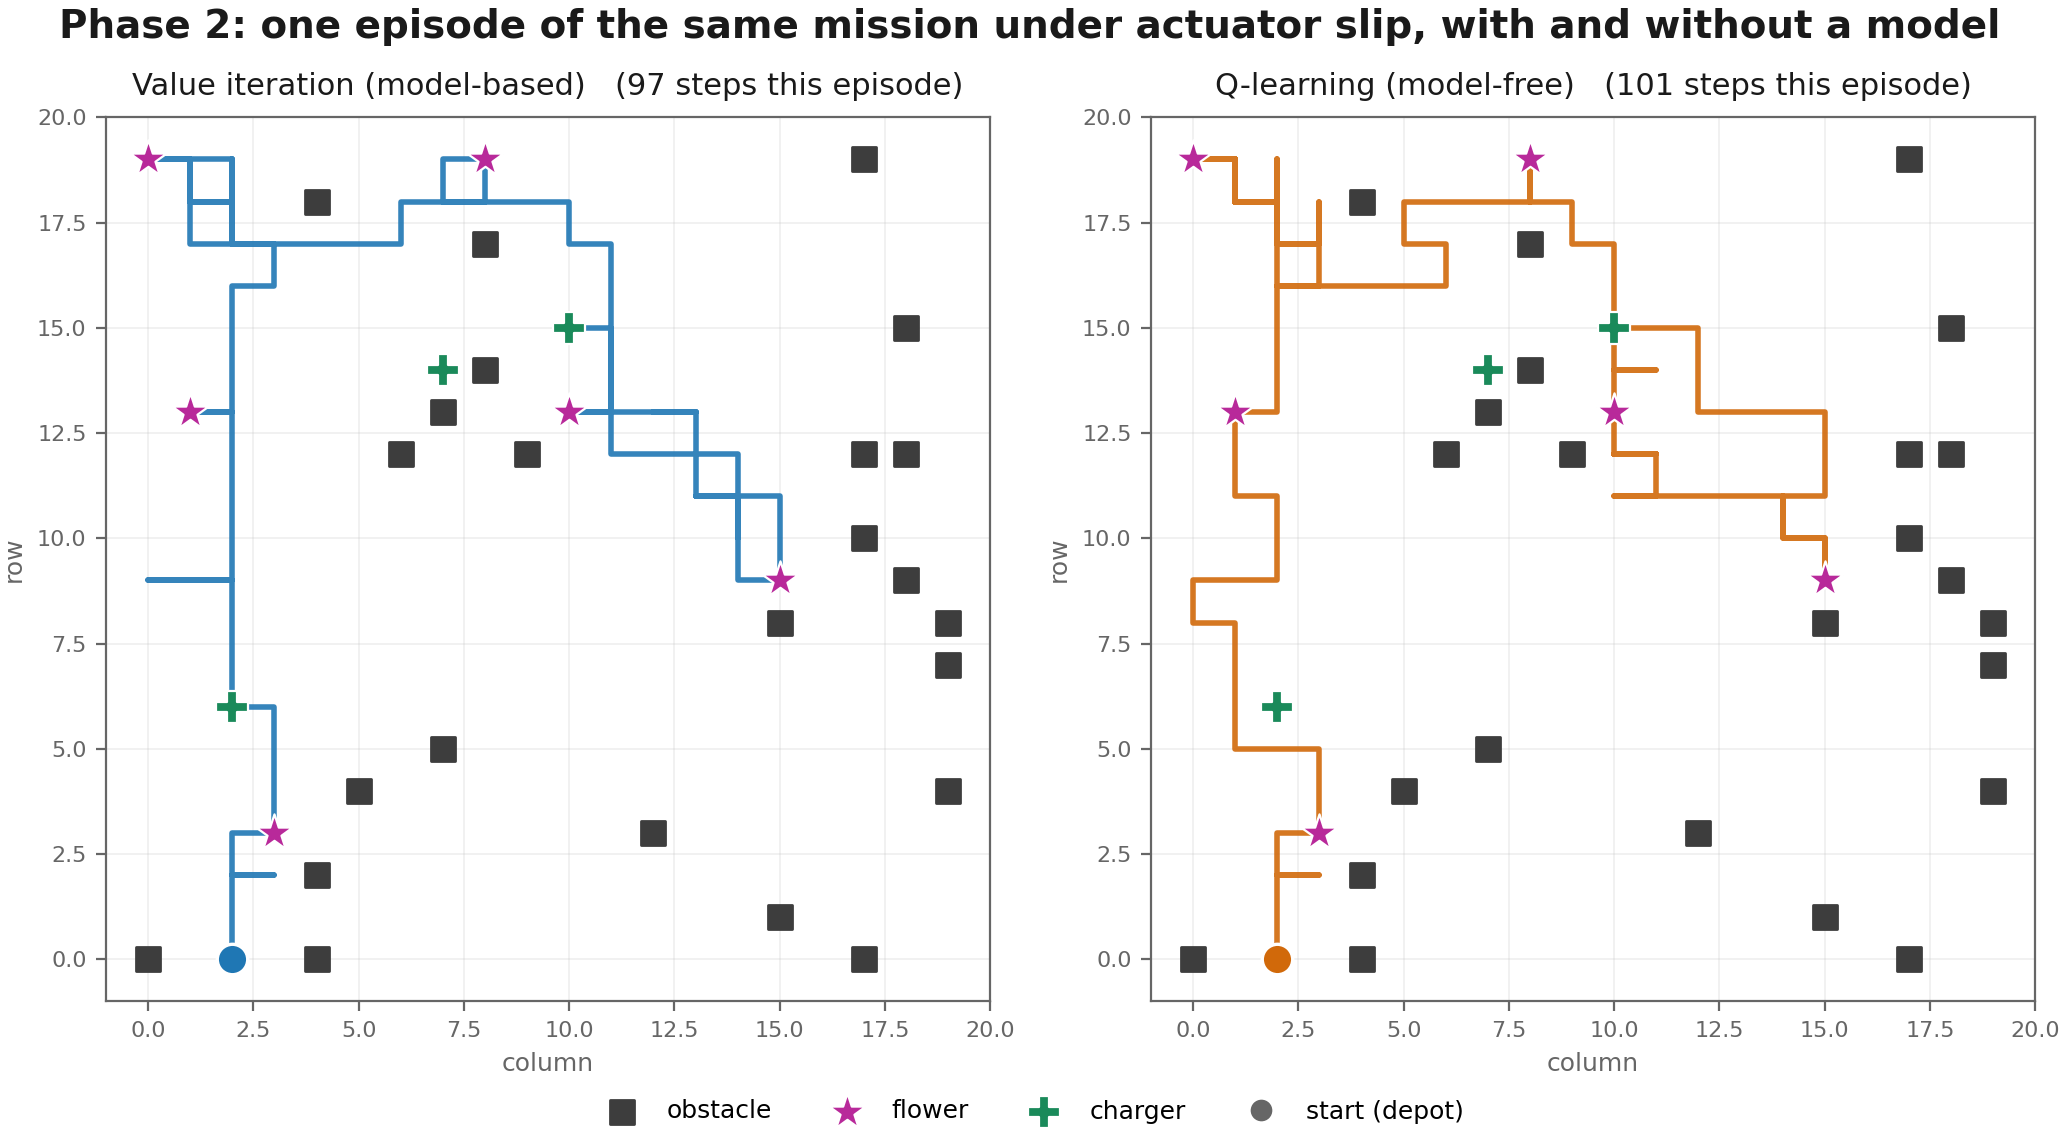
\includegraphics[width=0.85\textwidth]{cs3_vi_ql_paths.png}
\caption{CS-3 Phase 2: one episode of the same mission executed by each method
under the \emph{same} actuator-slip model, so the two panels are directly
comparable. Both pollinate every flower and return to a charger; the model-free
route is different in detail but equivalent in competence. Note that the
model-based route is \emph{also} ragged---the wandering is slip, not
inexperience.}
\label{fig:cs3paths}
\end{figure}

\begin{figure}[tp]
\centering
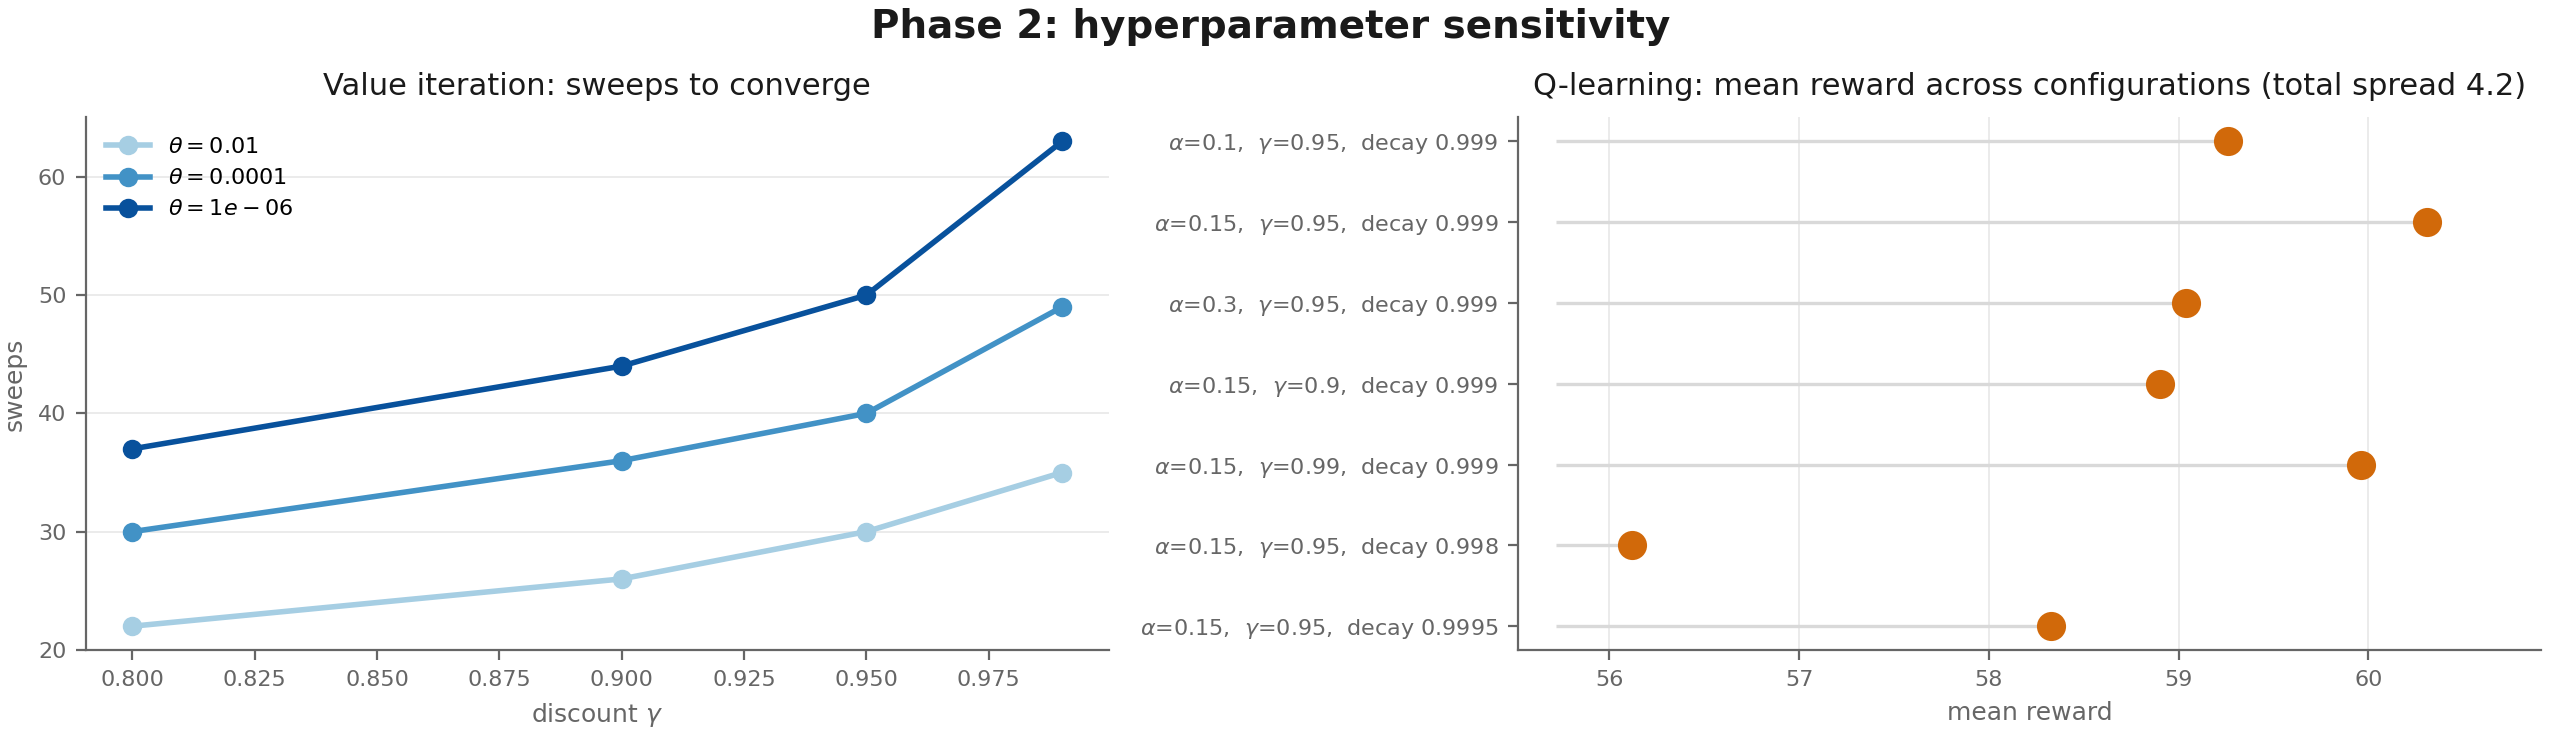
\includegraphics[width=\textwidth]{cs3_phase2_sensitivity.png}
\caption{CS-3 Phase 2 hyperparameter sensitivity. \emph{Left:} value iteration's
sweeps to convergence versus discount $\gamma$ at three residual thresholds
$\theta$; the recovered path stays at $63$--$65$ steps throughout, so the extra
sweeps buy precision in $V$, not a better policy. \emph{Right:} Q-learning's mean
reward across seven $(\alpha,\gamma,\varepsilon\text{-decay})$ configurations,
all within a $4.2$-reward band. Drawn as a dot plot rather than bars because the
claim is that the spread is \emph{small}, and bars on a non-zero baseline would
inflate it.}
\label{fig:cs3sens}
\end{figure}

\paragraph{Structural lesson.}
A huge, discrete, multi-objective assignment calls for \emph{population-based
metaheuristics}, and among them the family whose encoding matches the problem
(discrete GA) wins. A stochastic sequential-control problem calls for a
\emph{policy}, not a fixed plan; when the model is known, dynamic programming
delivers that policy essentially instantly (optimally per goal set, given the
sequential decomposition above), and when the model is absent, model-free RL is
the only option that runs at all.

%=======================================================================
\section{Cross-Case Synthesis}
\label{sec:synthesis}
%=======================================================================
Read together, the three case studies compose a single decision rule
(Table~\ref{tab:synth}). The controlling variables are the \emph{size and
observability} of the space, the presence of \emph{hard constraints}, and whether
outcomes are \emph{deterministic}.

\begin{table}[t]
\centering
\caption{The unifying decision rule distilled from the three case studies.}
\label{tab:synth}
\small
\renewcommand{\arraystretch}{1.3}
% Same budget as Table 1: 14.4cm of column plus 1.27cm of \tabcolsep.
\begin{tabular}{@{}p{3.15cm} p{3.95cm} p{3.95cm} p{3.35cm}@{}}
\toprule
\textbf{If the problem is\ldots} & \textbf{Structural cue} & \textbf{Right family} & \textbf{Evidence} \\
\midrule
Small, known, single path to a goal & Tractable state space, admissible heuristic available & Informed exact search (A$^\star$) & CS-1: optimal cost, $17\%$ fewer expansions than UCS \\
Combinatorial feasibility under many hard rules & Astronomical but \emph{structured} space & Backtracking $+$ inference $+$ MRV/LCV; min-conflicts for speed & CS-2: MRV turns a failed instance into $41$ nodes \\
Huge, discrete, multi-objective optimization & No gradient; $5^{400}$ candidates & Population metaheuristics (GA $>$ PSO when encoding fits) & CS-3.1: GA $1.43$ vs.\ PSO $1.60$ fitness ($10$ seeds) \\
Sequential control under uncertainty & Stochastic transitions, delayed reward & Dynamic programming if model known; model-free RL if not & CS-3.2: VI $176\times$ faster; QL matches it model-free \\
\bottomrule
\end{tabular}
\end{table}

Three cross-cutting observations tie the cases together. \textbf{First,
exploiting structure beats raw power at every scale}: an admissible heuristic
(CS-1), a variable-ordering heuristic (CS-2), a problem-matched encoding and a
seeded population (CS-3.1), and a known transition model (CS-3.2) each convert an
intractable or wasteful search into an efficient one. \textbf{Second, guarantees
have a price, and knowing when to pay it is the skill}: A$^\star$ and value
iteration buy optimality with a known space/model; greedy search, min-conflicts
and Q-learning surrender a guarantee for speed or for the ability to run at all
under partial knowledge. \textbf{Third, the ``best'' algorithm is objective- and
regime-dependent}: cost-based optimal search only overtakes heuristic-only search
once the priority makes the truly cheapest route non-obvious (CS-1), and value
iteration only beats Q-learning when a model exists (CS-3.2).

%=======================================================================
\section{Reproducibility}
%=======================================================================
Every result above is regenerated by fixed-seed, from-scratch Python scripts.
Each case study deterministically constructs its instance, runs its algorithms,
reports per-run metrics (to CSV for CS-3, to a console report for CS-1 and CS-2),
and renders the figures reproduced here. No
external solver or learning framework is used. Hard-constraint results (CS-2) are
re-verified by an independent constraint checker. The complete code, seeds, CSV
outputs and figure-generation scripts are publicly available at
\url{https://github.com/meavi44/ai-algorithm-families}, so that all tables and
figures can be reproduced from a single command per case study.

%=======================================================================
\section{Limitations and Future Work}
%=======================================================================
Our claims are scoped to the three implemented instances and should be read as an
illustrative, not exhaustive, mapping. \textbf{(1) Single instance per problem.}
The stochastic methods are averaged over $10$ seeds (Section~5), but all runs use
one fixed instance per case study. We report a significance test only for the
headline value-iteration/Q-learning reward comparison; the remaining comparisons
are argued from mean$\,\pm\,$std alone. A stronger study would randomize the
instances themselves---many greenhouses, road graphs and vehicle
populations---and test every comparison formally, to separate algorithm behaviour
from instance-specific quirks. \textbf{(2)
Synthetic data.} The greenhouse and (partially) the road/fuel instances are
synthetic; real telemetry would strengthen external validity. \textbf{(3) Modest
scales.} The navigation grid ($20\times20$) and vehicle counts ($n\le40$) are
small enough for exact methods; the crossover points we identify would shift at
larger scale. \textbf{(4) Fixed weightings.} Multi-objective terms use fixed
weights; a Pareto analysis would characterize the trade-offs more fully. Future
work will add multi-seed statistics, larger and real-world instances, and
additional family representatives (e.g.\ policy iteration, SARSA, ant-colony
optimization) to sharpen the structural mapping.

%=======================================================================
\section{Conclusion}
%=======================================================================
We advanced and tested a single thesis: problem structure should choose the
algorithm family. Three from-scratch, reproducible case studies---state-space
search, constraint satisfaction, and combined optimization/learning---each
confirmed it and, taken together, distilled into a compact decision rule.
Informed exact search dominates a small known space; constraint inference and
ordering heuristics tame a structured combinatorial one; population metaheuristics
handle enormous discrete optimization; and dynamic programming or model-free
reinforcement learning handle stochastic sequential control depending on whether a
model is available. The consistent thread is that \emph{recognizing structure, and
exploiting it, is what turns an intractable problem into a solved one}.

%=======================================================================
\begin{thebibliography}{99}
\small
\bibitem{russell2020} S.~Russell and P.~Norvig,
\emph{Artificial Intelligence: A Modern Approach}, 4th ed. Pearson, 2020.

\bibitem{hart1968} P.~E.~Hart, N.~J.~Nilsson, and B.~Raphael,
``A formal basis for the heuristic determination of minimum cost paths,''
\emph{IEEE Trans. Systems Science and Cybernetics}, vol.~4, no.~2, pp.~100--107, 1968.

\bibitem{pearl1984} J.~Pearl,
\emph{Heuristics: Intelligent Search Strategies for Computer Problem Solving}.
Addison-Wesley, 1984.

\bibitem{dechter2003} R.~Dechter,
\emph{Constraint Processing}. Morgan Kaufmann, 2003.

\bibitem{mackworth1977} A.~K.~Mackworth,
``Consistency in networks of relations,''
\emph{Artificial Intelligence}, vol.~8, no.~1, pp.~99--118, 1977.

\bibitem{minton1992} S.~Minton, M.~D.~Johnston, A.~B.~Philips, and P.~Laird,
``Minimizing conflicts: a heuristic repair method for constraint satisfaction and
scheduling problems,''
\emph{Artificial Intelligence}, vol.~58, no.~1--3, pp.~161--205, 1992.

\bibitem{cheeseman1991} P.~Cheeseman, B.~Kanefsky, and W.~M.~Taylor,
``Where the really hard problems are,''
in \emph{Proc. IJCAI}, 1991, pp.~331--337.

\bibitem{kennedy1995} J.~Kennedy and R.~Eberhart,
``Particle swarm optimization,''
in \emph{Proc. IEEE Int. Conf. Neural Networks}, 1995, pp.~1942--1948.

\bibitem{holland1975} J.~H.~Holland,
\emph{Adaptation in Natural and Artificial Systems}.
University of Michigan Press, 1975.

\bibitem{goldberg1989} D.~E.~Goldberg,
\emph{Genetic Algorithms in Search, Optimization, and Machine Learning}.
Addison-Wesley, 1989.

\bibitem{bellman1957} R.~Bellman,
\emph{Dynamic Programming}. Princeton University Press, 1957.

\bibitem{puterman1994} M.~L.~Puterman,
\emph{Markov Decision Processes: Discrete Stochastic Dynamic Programming}.
Wiley, 1994.

\bibitem{watkins1992} C.~J.~C.~H.~Watkins and P.~Dayan,
``Q-learning,'' \emph{Machine Learning}, vol.~8, no.~3--4, pp.~279--292, 1992.

\bibitem{sutton2018} R.~S.~Sutton and A.~G.~Barto,
\emph{Reinforcement Learning: An Introduction}, 2nd ed. MIT Press, 2018.
\end{thebibliography}

\end{document}
